% simple.tex -- a very simple thesis document for demonstrating
%   dalthesis.cls class file
\documentclass[12pt]{dalthesis}
\usepackage{dsfont}
\usepackage{caption}
\usepackage{subcaption}
\usepackage{float}
\usepackage{graphicx}

% ----------------------------------------------------------------------
% Packages.
\usepackage{amsmath,amsfonts,amsthm,amssymb}
\usepackage{braket}
\usepackage{mathdots}
\usepackage{mathtools}
\usepackage{tikz}
\usetikzlibrary{calc,decorations.pathreplacing,positioning,shapes}
\usepackage{hyperref}
\usepackage[capitalize]{cleveref}
\usepackage[normalem]{ulem}
\usepackage{qcircuit}
\usepackage{tikz-cd}
\usetikzlibrary{cd}
\usepackage{mleftright}
\usepackage{comment}
\newcommand{\note}[1]{{\color{red} #1}}

% ----------------------------------------------------------------------
% Some notation.

% Function restriction.
\newcommand\restrict[1]{\raisebox{-.5ex}{$|$}_{#1}}

% Residue of a matrix M.
\newcommand\mbar{\overline{M}}

% Matrix rings.
\newcommand{\matricesmn}[3]{\mathcal{M}_{#1\times #2}(#3)}
\newcommand{\matrices}[1]{\mathcal{M}(#1)}

\newcommand{\pauli}[1]{\mathcal{P}_{#1}}
\newcommand{\clifford}[1]{\mathcal{C}_{#1}}
\newcommand{\realclifford}[1]{\mathcal{C}_{#1}^{\mathbb{R}}}
\newcommand{\weight}{\operatorname{weight}}
\newcommand{\realpauli}[1]{\mathcal{P}_{#1}^{\mathbb{R}}}

% CNOT and SWAP gates.
\newcommand{\CNOT}{\mathrm{CNOT}}
\newcommand{\SWAP}{\mathrm{SWAP}}

% Matrices.
\newcommand{\diag}{\operatorname{diag}}

% Rings.
\newcommand{\Z}{\mathbb{Z}}
\newcommand{\N}{\mathbb{N}}
\newcommand{\F}{\mathbb{Z}_2}
\newcommand{\R}{\mathbb{R}}
\newcommand{\C}{\mathbb{C}}
\newcommand{\Zi}{\Z\left[i\right]}
\newcommand{\Zomega}{\Z\left[\omega\right]}
\newcommand{\Zrt}{\Z\left[\frac{1}{\sqrt{2}}\right]}
\newcommand{\Zrtwo}{\Z\left[\sqrt{2}\right]}
\newcommand{\Zrtwoi}{\Z[1/\sqrt{2},i]}
\newcommand{\Zint}{\Z\left[\sqrt{2}\right]}
\newcommand{\rtZrt}{\frac{1}{\sqrt{2}^k}\Z\left[\sqrt{2}\right]}

% Norm and adjoint.
\newcommand{\norm}[1]{\left\lVert#1\right\rVert}

% Misc math notation.
\newcommand{\inv}{^{-1}}
\newcommand{\s}[1]{\{#1\}}

\newcommand{\Stab}{\mathrm{Stab}}


% ----------------------------------------------------------------------
% Theorem like environments.
\theoremstyle{plain}
\newtheorem{theorem}{Theorem}[section]
\newtheorem{lemma}[theorem]{Lemma}
\newtheorem{proposition}[theorem]{Proposition}
\newtheorem{corollary}[theorem]{Corollary}
\theoremstyle{definition}
\newtheorem{definition}[theorem]{Definition}
\newtheorem{example}[theorem]{Example}

\theoremstyle{remark}
\newtheorem{remark}[theorem]{Remark}

% ----------------------------------------------------------------------
% Macros for bibliography.

\newcommand{\urlalt}[2]{\href{#2}{\nolinkurl{#1}}}
\newcommand{\arxiv}[1]{\urlalt{arXiv:#1}{http://arxiv.org/abs/#1}}

%----------------------------------------------------------------------
% A hack: \m is similar to \vcenter, but works better.
% \mp{0.2}{x}: raise the box x so that 20% of it is below the
% centerline. Unlike \vcenter, don't change the horizontal spacing.

\newlength{\localh}
\newlength{\locald}
\newbox\mybox
\def\mp#1#2{\scalebox{0.8}{\setbox\mybox\hbox{#2}\localh\ht\mybox\locald\dp\mybox\addtolength{\localh}{-\locald}\raisebox{-#1\localh}{\box\mybox}}}
\def\m#1{\mp{0.5}{#1}}


\begin{document}

\title{Lower Bounds non-Clifford Resources}
\author{Ravi Rai}

% The following degrees are included in the current dalthesis.cls
% class file:
\mcs  % options are \mcs, \macs, \mec, \mhi, \phd, and \bcshon

% If you degree is not included, you can set several options manually.
% The following example shows the parameters for the \mcs degree.
% However, if you need to set these parameters manually, please check
% the correct names with the Faculty of Graduate Studies, and let the
% maintainer of this class file know (Vlado Keselj, vlado@cs.dal.ca).
% MCS Example:

\degree{Master of Science}
\degreeinitial{M.Sc.}
\faculty{Computer Science}
\dept{Faculty of Computer Science}

% Month and Year of Defence
\defencemonth{August}\defenceyear{2021}

\dedicate{\ldots}

% This sample thesis contains no tables nor figures, so there is no
% need to include lists of tables and figures in the front matter:
\nolistoftables
\nolistoffigures

\frontmatter

\begin{abstract}
\ldots
\end{abstract}

\begin{acknowledgements}
\ldots
\end{acknowledgements}

\mainmatter

\chapter{Introduction}

\ldots

\chapter{The Stabilizer Formalism}
\section{Basics}
%To begin, we need to introduce and develop the formalism of stabilizer operators and its related quantities, but first some  basic definitions, starting with the Pauli matrices.

\begin{definition}
The \emph{Pauli matrices} $X$, $Y$, and $Z$ are defined as:
  \[
  X= \begin{bmatrix}
    0 & 1 \\
    1 & 0
  \end{bmatrix}, \quad
  Y = \begin{bmatrix}
  0 & -i \\
  i & 0
  \end{bmatrix}, \quad \mbox{and} \quad
  Z = \begin{bmatrix}
  1 & 0 \\
  0 & -1
  \end{bmatrix}.
  \]
\end{definition}

We write $A \otimes B$ for the tensor product of two matrices $A$ and $B$. If S is a set of matrices then $M^{\otimes n}$ is the set of matrices comprised of tensor products of elements ins $M$.

\begin{definition}
\label{PauliGroup}
The \emph{Pauli group on $n$ qubits} $\mathcal{P}(n)$ is the matrix group with elements $\{ \pm I, \pm X, \pm Y, \pm Z, \pm iI, \pm iX, \pm iY, \pm iZ \}^{\otimes n}$.
\end{definition}

Note that the $\pm 1$ and $\pm i$ factors in the elements of $\mathcal{P}(n)$ ensures the closure of the group.

\begin{definition}
For $P \in \mathcal{P}(1)$, we write $P_j$ for $I \otimes \dots \otimes I \otimes P \otimes I \dots \otimes I$.
\end{definition}

\begin{proposition}
We have $|\mathcal{P}(n)|=4^{n+1}$.
\end{proposition}

\begin{proof}
By induction, first let $n=1$. Then from definition \ref{PauliGroup} we see that there are $16 = 4^2$ elements in $\mathcal{P}(1)$, so the base case is true. Now assume that the statement is true for $m$ qubits, i.e. $|\mathcal{P}(m)| = 4^{m+1}$. Then $\mathcal{P}(m+1)$ has elements that are tensor products of elements in $\mathcal{P}(m)$ and $I$, $X$, $Y$, and $Z$. Thus there are $4 \cdot 4^{m+1} = 4^{(m+1)+1}$ elements in $\mathcal{P}(m+1)$. Note that we only count these tensor products since e.g., $P \otimes -iX = P' \otimes X$ where $P' = -iP$, for $P, P' \in \mathcal{P}(m)$.
\end{proof}

\begin{definition}
Let $\ket{\psi}$ be a quantum state and $U$ be an operator, then we say that $\ket{\psi}$ is \emph{stabilized} by $U$ if $U\ket{\psi} = \ket{\psi}$. 
\end{definition}

\begin{definition}[Stabilizer]
Let $\ket{\psi}$ be a non-zero $n$-qubit state. The \emph{stabilizer} of $\ket{\psi}$ is the subgroup $\mathcal{P}(n)$ for which $\ket{\psi}$ is a $+1$ eigenstate, and is denoted by Stab$\ket{\psi}$. 
\end{definition}

This means that Stab$\ket{\psi}$ = $\{P \in \mathcal{P}(n) \: P \ket{\psi} = \ket{\psi} \}$.  States for which the stabilizer contains only the identity matrix are said to have a trivial stabilizer. 

\begin{definition}[Stabilizer States]
Let $\ket{\psi}$ be a state for which the size of its stabilizer is $2^n$. The we call $\ket{\psi}$ a stabilizer state.
\end{definition}

The reason behind using this stabilizer formalism is that we can easily describe many quantum states by working with operators that stabilize them, rather than by explicitly working with the states themselves. A key component to making use of the stabilizer formalism lies in the Pauli group $\mathcal{P}(n)$ defined above. Next are a few propositions regarding the stabilizer.

\begin{proposition}
\label{stabilizerfacts}
Let $\ket{\psi}$ be a non-zero n qubit state. Then we have the following facts about Stab$\ket{\psi}$:
\begin{enumerate}
\item Stab$\ket{\psi}$ does not contain -$I$.
\item All Pauli group elements contained in Stab$\ket{\psi}$ commute with each other and are Hermitian matrices.
\item The size of the stabilizer is equal to some power of two.
\item Given any Clifford Unitary $C$, the size of Stab$\ket{\psi}$ is always equal to the size of Stab$(C \ket{\psi})$.
\item Finally, the size of the stabilizer is multiplicative for the tensor products of states, that is $| \text{Stab} (\ket{\psi} \ket{\phi})| = |\text{Stab}\ket{\psi}| \cdot |\text{Stab}\ket{\phi}|$. 
\end{enumerate}
\end{proposition}

\begin{proof}
\hspace{20mm}
\begin{enumerate}
\item If $\-I \in \text{Stab}\ket{\psi}$, then $-\ket{\psi} =-I\ket{\psi} = \ket{\psi}$, which of course is not true for non-zero states.

\item First note that for any two Pauli's $P, Q$, they either commute or anti-commute. Now suppose $P, Q \in \text{Stab}\ket{\psi}$ anti-commute. Then $\ket{\psi} = PQ\ket{\psi} = -QP\ket{\psi} = -\ket{\psi}$. This implies that $-I \in \text{Stab}\ket{\psi}$, which from above can't be true, so $P$ and $Q$ must commute.

\item It is known that the Pauli group's cardinality is a power of two, and since $\text{Stab}\ket{\psi}$ is a subgroup of the Pauli group, $|\text{Stab}\ket{\psi}|$ must divide a power of two, thus it must also be a power of two.

\item First note that Clifford unitaries normalize pauli matrices, i.e. for some Clifford unitary $C$, and some pauli $P$, $CPC^{\dag} = P'$, where $P'$ is also a pauli. Now let $P \in \text{Stab}\ket{\psi}$ and let $C$ be some Clifford unitary. Then $P'C\ket{\psi} = CPC^{\dag}C\ket{\psi} = CP\ket{\psi} = C\ket{\psi}$, so $P' \in \text{Stab}(C\ket{\psi})$. Now consider the map $\theta_C : \text{Stab}\ket{\psi} \rightarrow \text{Stab}(C\ket{\psi})$ which takes elements $P \mapsto CPC^{\dag} = P'$. This map has an inverse, $\theta_{C^\dag}: \text{Stab}(C\ket{\psi}) \longrightarrow \text{Stab}(C^{\dag}C\ket{\psi})$, which takes elements $P' \mapsto C^{\dag}P'C$ (where we note that $\text{Stab}(C^{\dag}C\ket{\psi}) = \text{Stab}\ket{\psi}$). Thus $\theta_C$ is a bijection, and so we have that $|\text{Stab}\ket{\psi}| = |\text{Stab}(C\ket{\psi})|$.

\item Let $\ket{\phi}$ be another non-zero state on n qubits, and let $P \in \text{Stab}\ket{\psi}$ and $Q \in \text{Stab}\ket{\phi}$. Then $P \otimes Q \ket{\psi}\ket{\phi} = P\ket{\psi} \otimes Q\ket{\phi} = \ket{\psi}\ket{\phi}$. So $P \otimes Q \in \text{Stab}\ket{\psi}\ket{\phi}$. Now let $R \in \text{Stab}\ket{\psi}\ket{\phi}$. Then since $R$ is a Pauli, we can write $R = R_1 \otimes R_2$, and $R\ket{\psi}\ket{\phi} = \ket{\psi}\ket{\phi} = R_1 \otimes R_2 \ket{\psi}\ket{\phi} = R_1\ket{\psi} \otimes R_2\ket{\phi}$. Now let $\ket{\psi '} = R_1\ket{\psi}$ and $\ket{\phi '} = R_2\ket{\phi}$, and since $R_1$ and $R_2$ are both Clifford unitaries, fact 4 gives us that $|\text{Stab}\ket{\psi '}| = |\text{Stab}(R_1\ket{\psi})|$ and $|\text{Stab}\ket{\phi '}| = |\text{Stab}(R_2\ket{\phi})|$. We also have that $|\text{Stab}(R\ket{\psi}\ket{\phi})| = |\text{Stab}\ket{\psi '}\ket{\phi '}|$.


 So every element in $\text{Stab}\ket{\psi}\ket{\phi}$ is of the form $R_1 \otimes R_2$ as above, thus $\text{Stab}\ket{\psi}\ket{\phi} = \text{Stab}\ket{\psi} \otimes \text{Stab}\ket{\phi}$. Then we have a bijection (from the direct product) $\theta:\text{Stab}\ket{\psi} \times \text{Stab}\ket{\phi} \longrightarrow  \text{Stab}\ket{\psi} \otimes \text{Stab}\ket{\phi}$, which gives us $|\text{Stab}\ket{\psi}\ket{\phi}| = |\text{Stab}\ket{\psi} \otimes \text{Stab}\ket{\phi}| = |\text{Stab}\ket{\psi}| \cdot |\text{Stab}\ket{\phi}|$.
\end{enumerate}
\end{proof}



An example of a stabilizer state is the $\ket{0}$ state, since there are $2^1$ pauli's that stabilize it, namely $I$ and $Z$. Note that, from fact 4 in Proposition \ref{stabilizerfacts}, for any Clifford $C$, $|\text{Stab}\ket{0}| = |Stab(C\ket{0})| = 2^1 \implies C\ket{0}$ is a stabilizer state. And an example of a non-stabilizer state is $\ket{\psi} = \frac{1}{\sqrt{2}}(\ket{00} + \frac{i}{2} \ket{11})$, which through computation one can find that it has the following stabilizers: $I \otimes I$ and $Z \otimes Z$. Since there are only $2$ stabilizers, and $2 \neq 2^2$, $\ket{\psi}$ cannot be a stabilizer state.

\begin{corollary}
The computational basis state $\ket{00 \dots 0}$ on n-qubits is a stabilizer state. If $\ket{\psi}$ is a basis state, then it is a stabilizer state. 
\end{corollary}
\begin{proof}
First we prove that $\ket{00 \dots 0}$ is a stabilizer state by induction, where the base case is the $\ket{0}$ state which we know is a stabilizer state from above (and $|\text{Stab}\ket{0}| = 2^1$). Now assume that $\ket{00 \dots 0}$ is a stabilizer state on n-qubits with $|\text{Stab}\ket{00 \dots 0}| = 2^n$. Let $P \in \text{Stab}\ket{0}$ and $Q \in \text{Stab}\ket{00 \dots 0}$, then $(P \otimes Q)\ket{0}\ket{00 \dots 0} = P\ket{0} \otimes Q\ket{00 \dots 0} = \ket{0}\ket{00 \dots 0} = \ket{00 \dots 00}$ (n+1 qubits). So $P \otimes Q \in \text{Stab}\ket{00 \dots 00}$, and from above arguments we know that every element in $\text{Stab}\ket{00 \dots 00}$ is of this form, thus there are $2^{n+1}$ elements in $\text{Stab}\ket{00 \dots 00}$, making it a stabilizer state.


Next, if $\ket{\psi}$ is an $n$-qubit basis state, then it differs from the $n$-qubit computational basis state $\ket{00 \ldots 0}$ by only a Clifford unitary, i.e. $C\ket{00 \ldots 0} = \ket{\psi}$ for some Clifford circuit C. Then as remarked above, it follows that $\ket{\psi}$ is a stabilizer state.
\end{proof}

\begin{theorem}
If $\ket{\psi}$ is a stabilizer state, then there is a circuit $C$ such that $C\ket{\psi} = \ket{00 \dots 0}$.
\end{theorem}
\begin{proof}
By Theorem 8 in \cite{}, every stabilizer state can be represented by a tableau, which can then be converted into a tableau that represents the $\ket{00 \dots 0}$ state using only Clifford operations. Applying these Clifford operators is equivalently applying Clifford operators to the appropriate qubits of $\ket{\psi}$, thus resulting in a Clifford circuit $C$ such that $C\ket{\psi} = \ket{00 \dots 0}$. 
\end{proof}

\begin{theorem}
If $\ket{\psi}$ is an $n$-qubit stabilizer state, then $\textit{Stab}\ket{\psi}$ uniquely determines $\ket{\psi}$.
\end{theorem}
\begin{proof}
First note that each $P \in \textit{Stab}\ket{\psi}$ imposes the linear constraint that $P\ket{\psi} = \ket{\psi}$ on the $2^n$-dimensional vector space. The subspace of vectors that satisfy this constraint has half of this space, meaning that it has dimension $2^{n-1}$. Let gen($\ket{\psi}$) be the set of generators for $\textit{Stab}\ket{\psi}$, where we add independent generators to gen($\ket{\psi}$) one by one. This way we subsequently half the dimension of the vector subspace that satisfies all the linear constraints, and since $|\textit{gen}(\ket{\psi})| = n$, this dimension reduces to $1$. Thus there is only one possible vector and so $\ket{\psi}$ is uniquely determined.
\end{proof}

\begin{definition}
Let $S$ be a subgroup of $\mathcal{P}(n)$, and let $V_S$ be the set of $n$ qubit states which are fixed by every element of $S$. $V_S$ is the vector space stabilized by $S$, and we call $S$ the stabilizer of the space $V_S$. 
\end{definition}

We can also make use of the Pauli groups generators, where to check if a particular vector is stabilized by a group $S$, checking if the generators stabilize it will be sufficient.


\begin{proposition}
Let $S$ be a subgroup of $\mathcal{P}(n)$ and $V_S$ its associated vector space stabilized by $S$. Then if $V_S$ is not trivial $S$ is a commutative group that does not contain $-I$.
\end{proposition}
\begin{proof}
Consider the subgroup $\{\pm I, \pm X \}$ of $\mathcal{P}(1)$. Obviously the only solution to $(-I)\ket{\psi} = \ket{\psi}$ is $\ket{\psi} = 0$, and so $\{\pm I, \pm X \}$ stabilizes the trivial vector space. An immediate consequence of this is that we need $-I$ to not be an element of $S$. Furthermore, all elements of $S$ must commute, because if they did not then they would anti-commute, so $-I$ would necessarily be an element of the group.
\end{proof}


\begin{proposition}
Let $S = \langle g_1, \dots , g_{n-k} \rangle$ be generated by $n-k$ independent and commuting elements from $\mathcal{P}(n)$, and such that $-I \not \in S$. Then $V_S$ is a $2^k$ - dimensional vector space.
\end{proposition}


\section{Relating Unitaries}
Now we describe how unitaries relate to the stabilizer formalism, starting with a proposition. 
\begin{proposition}
$Stab(\ket{\psi}) = \langle g_1 , \dots , g_n \rangle \Longrightarrow Stab(U\ket{\psi}) = \langle Ug_1U^{\dag}, \dots , Ug_lU^{\dag} \rangle$
\end{proposition}
\begin{proof}
First, suppose we apply a unitary operations $U$ to a vector space $V_S$ stabilized by the subgroup $S$ as before, and let $\ket{\psi} \in V_S$. Note that $S = Stab(\ket{\psi})$. Then for any $g \in S$, $U\ket{\psi} = Ug\ket{\psi} = UgU^{\dag}U\ket{\psi}$. Thus, the state $U\ket{\psi}$ is stabilized by $UgU^{\dag}$, and so the vector space $UV_S$ is stabilized by the group $USU^{\dag}$. Furthermore, if $g_1, \dots , g_l$ generate $S$, then $Ug_1U^{\dag}, \dots , Ug_lU^{\dag}$ generates $USU^{\dag}$.
\end{proof}

There is a particularly appealing and advantageous form that special unitary operations take on. For us, the Hadamard and phase gates are nice examples to consider. We define them now, along with the CNOT gate which will be used later on.

\begin{definition}
The Hadamard ($H$), phase ($S$) and controlled-NOT (CNOT) gates are defined as follows:
\begin{equation}
H = 
\frac{1}{\sqrt{2}} 
\begin{bmatrix}
1 & 1 \\
1 & -1
\end{bmatrix}, \quad
S = 
\begin{bmatrix}
1 & 0 \\
0 & i
\end{bmatrix}, \quad \mbox{and} \quad
CNOT = 
\begin{bmatrix}
1 & 0 & 0 & 0 \\
0 & 1 & 0 & 0 \\
0 & 0 & 0 & 1 \\
0 & 0 & 1 & 0
\end{bmatrix}.
\end{equation}
\end{definition}


\begin{proposition}
$H$ and $S$ act on Paulis as follows:
\begin{center}
$HXH^{\dag} = Z$ and $HZH^{\dag} = X$, $SXS^{\dag} = Y$ and $SZS^{\dag} = Z$.
\end{center}
Note that we need not specify the action on $Y$ since $Y = iXZ$, so the action on $X$ and $Z$ gives and fixes the action on $Y$.
\end{proposition}


The state $\ket{0}$ is stabilized by $Z$, and after applying the Hadamard to $\ket{0}$ to get the new state $\ket{+}$, we see that it is now stabilized by $X$. The power in this example can be seen once you consider the general $n$ qubit case. Consider the state $\ket{0}^{\otimes n}$ whose stabilizer is $\langle Z_1, Z_2, \dots , Z_n \rangle$. Then applying the Hadamard to each of of the $n$ qubits gives a state with stabilizer $\langle X_1 , X_2, \dots , X_n \rangle $. Now, observe that the final state vector here requires $2^n$ amplitudes to be specified, compared with the description provided by the generators: $\langle X_1, \dots , X_n \rangle$, which is linear in $n$. 

You can see that there is no entanglement in the quantum computer here, after applying the Hadamard to each qubit. This may lead to thinking that this stabilizer formalism is not so useful, however this changes when you see that there is an efficient description of the controlled-NOT gate, which together with the Hadamard gate can create entanglement. 

It turns out that there is a theorem that says that any unitary operation that takes elements of $\mathcal{P}(n)$ to elements of $\mathcal{P}(n)$ under conjugation can be composed of Hadamard, phase and controlled-NOT gates (proved later). This brings us to what we call the Clifford hierarchy. The Pauli group defines the $1st-level$ of the Clifford Hierarchy, which is $\mathcal{C}^{(1)} = e^{i\theta} \cdot \{I, X, Y, Z\}^{\otimes n}$, so it is $\mathcal{P}(1)$ but with all phases. The aforementioned group of automorphisms of the Pauli group is the $2nd-level$ of the Clifford Hierarchy, $\mathcal{C}^{(2)}$, and is also known as both the Clifford Group and the normalizer of $\mathcal{P}(n)$. We now define the $k^{th}-level$ of the Clifford Hierarchy, and follow it with an aforementioned theorem.

\begin{definition} The k-th level of the Clifford Hierarchy is:
\label{CliffHierarchy}
\begin{equation}
\mathcal{C}^{(k)} = \{ U | UPU^{\dag} \in \mathcal{C}^{(k-1)}, \forall P \in \mathcal{P}(n) \}
\end{equation}
\end{definition}

\begin{theorem}
Let $U \in \mathcal{C}^{(2)}$, then up to a global phase $U$ may be composed of $H$, $S$, and $CNOT$ gates.
\end{theorem}
\begin{proof}
We proceed by induction on $n$, the number of qubits.
Let $U$ be a single qubit unitary operator such that for $P \in \mathcal{P}(1)$, $UPU^{\dag} \in \mathcal{P}$. So $UPU^\dag = Q$ for some $Q \in \mathcal{P}(1)$. Since conjugation by $U$ on $P$ essentially acts as an automorphism map, observe that $P, Q \not\in \{iX, iY, iZ\}$, since for example $X^2 = I$ so $(UXU^\dag )^2 = I$, but if $X \mapsto iX = Q$, then we will have $I = (UXU^\dag)^2 = (iX)^2 = -I$, which is obviously not true. Moreover, we also have that $P \neq iI$ and $P \neq I$.

Now, suppose $U$ is an $n+1$ qubit gate in $N(G_{n+1})$ such that $UZ_1U^{\dag} = X_1 \otimes g$ and $UX_1U^{\dag} = Z_1 \otimes g'$ for some $g, g' \in G_n$.
Define a circuit $C$ as:
\begin{center}
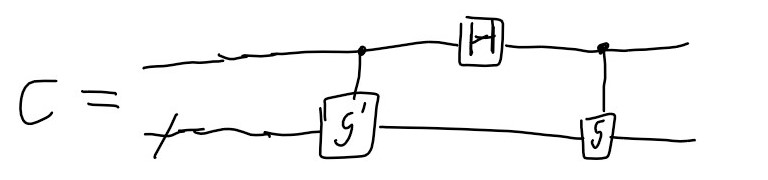
\includegraphics[scale = 0.5]{CliffordCircuitDef}
\end{center}
Now observe that $CZ_1C^{\dag} = X_1 \otimes g$ as follows:
\begin{center}
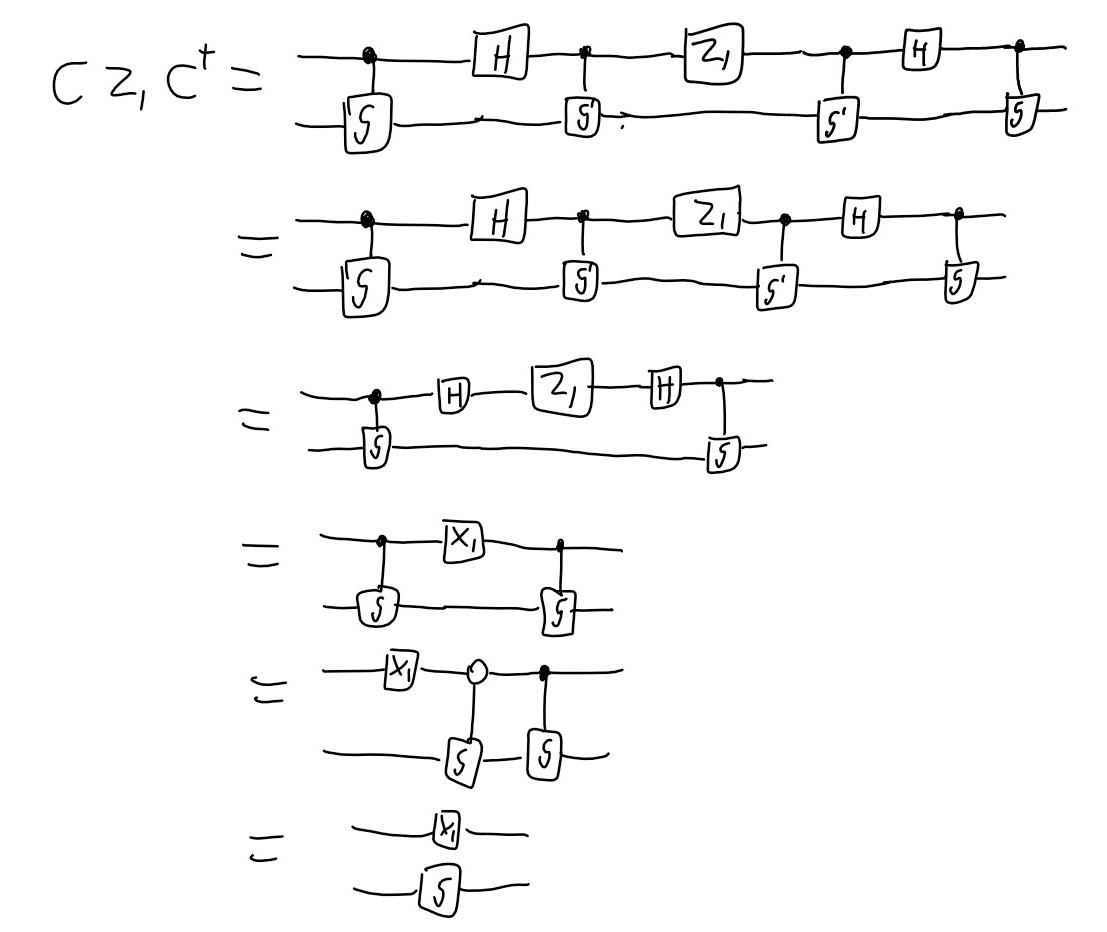
\includegraphics[scale = 0.5]{CZC}
\end{center}

Note that $g$ and $g'$ commute, as can be seen below:
\begin{align}
X_1Z_1 \otimes gg' &= (X_1 \otimes g)(Z_1 \otimes g') \\
 &= UZ_1U^{\dag}UX_1U^{\dag} \\ 
 &= -UX_1Z_1U^\dag \\
 &= -UX_1U^\dag UZ_1U^\dag \\ 
 &= -(Z_1 \otimes g')(X_1 \otimes g) \\
 &= -(Z_1X_1 \otimes g'g) \\
 &= X_1Z_1 \otimes g'g \\
\end{align}
Then we have that $I \otimes gg' = I \otimes g'g$, so applying the inverse of $I \otimes gg'$ to both sides, we have:
\begin{align}
I_{n+1} &= (I \otimes g'g)(I \otimes gg')^{-1} \\
 &= (I \otimes g'g)(I \otimes g'^{-1}g^{-1}) \\ 
 &= I \otimes g'gg'^{-1}g^{-1} \\
\end{align}
where $I_{n+1}$ is the identity on $n+1$ qubits. This implies that $g'gg'^{-1}g^{-1} = I_n$, thus $g'g = gg'$.

Now we make use of this commutation to show that $CX_1C^\dag = Z_1 \otimes g'$:
\begin{center}
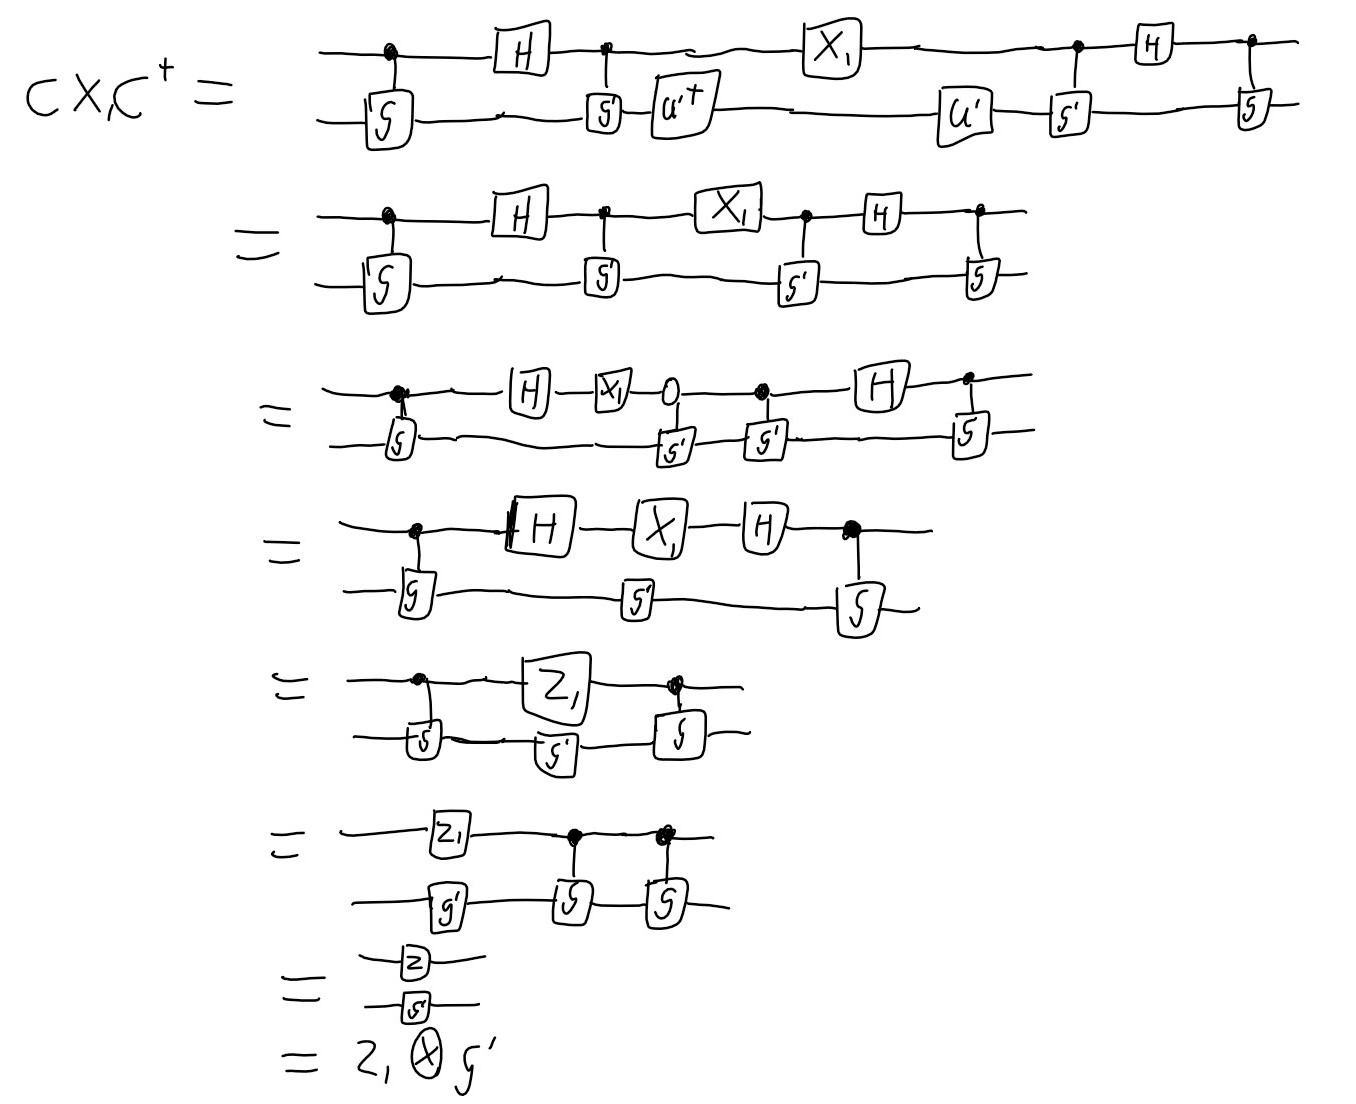
\includegraphics[scale = 0.5]{CXC}
\end{center}
Consider $U':= C^\dag U$. Then 
\begin{center}
$U'X_1U'^\dag = C^\dag U X_1 U^\dag C = C^\dag (Z_1 \otimes g') C = X_1$
\end{center} and 
\begin{center}
$U'Z_1U'^\dag = C^\dag U Z_1 U^\dag C = C^\dag (X_1 \otimes g) C = Z_1$
\end{center}
so $U' \in \mathcal{C}^{(2)}$.

Now let $U \in \mathcal{C}^{(2)}(n+1)$ so $UX_1U^\dag = P$ and $UZ_1U^\dag = Q$ for some $P, Q \in \mathcal{P}(n+1)$. Then we can write $P = P_1 \otimes g$ and $Q = Q_1 \otimes g'$ for $g, g' \in \mathcal{P}(n)$. From the inductive step, we can conjugate $UX_1U^\dag = P$ with some circuit $C$, which is comprised of only Hadamards and phase gates, such that 
\begin{center}
$CUX_1U^\dag C^\dag = CPC^\dag = C(P_1 \otimes g)C^\dag = Z_1 \otimes g$
\end{center}
and 
\begin{center}
$CUZ_1U^\dag C^\dag = CQC^\dag = C(Q_1 \otimes g')C^\dag = X_1 \otimes g'$
\end{center}
Let $u' = CU$, then by the inductive step, $U' \in \mathcal{C}^{(2)}(n)$. Next we repeat this process on $U'$ to get a $U'' = C'U' \in \mathcal{C}^{(2)}(n-1)$. Continue this process until we have a $U^{(n+1)'} = U^{n'}C^{n'} \in \mathcal{C}^{(2)}(1)$. Then $U = C^\dag U'$, but $U' = C'^\dag U''$, so $U = C^\dag C'^\dag U''$. Continuing this process results in 
\begin{center}
$U = C^\dag C'^\dag C''^\dag \cdots C^{n' \dag} U^{(n+1)'}$
\end{center}
Thus $U$ is a product of components comprised of only $H$ and $S$ gates, so it is as well (note $U^{(n+1)'}$ is a one-qubit Clifford so we know it is comprised of only $H$ and $S$ gates from the base case).
\end{proof}

\section{Measurements}
Yet another benefit of the stabilizer formalism shows up in the topic of measurements, specifically because we can quite easily describe measurements in the computational basis. Consider a $g \in \mathcal{P}(n)$, and imagine we make a measurement on it. Recall this means that $g$ is a Hermitian operator and is a product of Pauli's, and also for convenience let it not have any multiplicative factor of $-1$ or $\pm i$. Letting our system be in some state $\ket{\psi}$ with stabilizer $\langle g_1, \dots , g_n \rangle $, how does the stabilizer of the state transform under measurement? 

\begin{proposition}
Given a state $\ket{\psi}$ and Pauli $g$, after measurement the state transforms into $(I + g)\ket{\psi}/\sqrt{2}$ when the $+1$ result occurs, and $(I - g)\ket{\psi}/\sqrt{2}$ when the $-1$ result occurs, with probabilities $p(+1) = p(-1) = 1/2$.
\end{proposition}

\begin{proof}
We have two possible scenario's to consider, the first of which is when $g$ commutes with all generators. Observe that $g_jg\ket{\psi} = gg_j\ket{\psi} = g\ket{\psi}$ for each stabilizer generator, so $g\ket{\psi}$ is in $V_S$ and is thus a multiple of $\ket{\psi}$. Because $g^2 = I$, $g\ket{\psi} = \pm\ket{\psi}$, so either $g$ or $-g$ must be in the stabilizer. It follows that either $g$ or $-g$ is an element of the stabilizer. Suppose $g$ is in the stabilizer, then $g\ket{\psi} = \ket{\psi}$ and so a measurement of $g$ yields $+1$ with probability one, and the measurement leaves the stabilizer invariant. The argument for $-g$ being in the stabilizer follows similarly.

The second scenario is when $g$ anti-commutes with one or more generators. Without loss of generality let $g$ anti-commute with $g_1$, and commute with all other generators. Note that if $g$ did anti-commutes with another generator, say $g_2$, then it does commute with $g_1g_2$, and so you could just replace the generator $g_2$ with $g_1g_2$ in the stabilizer of $\ket{\psi}$. Also, $g$ has eigenvalues $\pm 1$ and so the projectors for the measurements outcomes are $(I \pm g)/2$ respectively, so we have measurement probabilities:
\begin{center}
$p(+1) = tr(\frac{I+g}{2}\ket{\psi}\bra{\psi})$
\end{center}
and 
\begin{center}
$p(-1) = tr(\frac{I-g}{2}\ket{\psi}\bra{\psi})$
\end{center}
Now, using the equalities $g_1\ket{\psi} = \ket{\psi}$ and $gg_1 = -g_1g$, and the cyclic property of the trace, we get:
\begin{center}
$p(+1) = tr(\frac{I+g}{2}g_1\ket{\psi}\bra{\psi}) = tr(g_1\frac{I-g}{2}g_1\ket{\psi}\bra{\psi}) = tr(\frac{I-g}{2}\ket{\psi}\bra{\psi}g_1)$
\end{center}
Since $g_1 = g_1^{\dag}$ and $\bra{\psi}g_1 = \bra{\psi}$ we have that:
\begin{center}
$p(+1) = tr(\frac{I-g}{2}\ket{\psi}\bra{\psi}) = p(-1)$.
\end{center}
Moreover, $p(+1) + p(-1) = 1$, so $p(+1) = p(-1) = 1/2$. So when the $+1$ result occurs, the new state of the system will be $(I + g)\ket{\psi}/\sqrt{2}$ with stabilizer $\langle g, g_2, \dots , g_n \rangle$ and probability $1/2$. And similarly, when the $-1$ result occurs, the state will be $(I - g)\ket{\psi}/\sqrt{2}$ with stabilizer $\langle -g, g_2, \dots , g_n \rangle$ and probability $1/2$.
\end{proof}

It is important to note that circuits made from only gates in $\mathcal{C}^{(2)}$ are not universal for quantum computing. To get around this issue, we can use gates from the $3rd-level$ of the Clifford Hierarchy: $\mathcal{C}^{(3)} = \{ U | UPU^{\dag} \in \mathcal{C}^{(2)}, \forall P \in \mathcal{P}(n)$, and so we will use unitaries from $\mathcal{C}^{(3)}$ frequently.

Two gates that are commonly used, including in this paper, that are not in the normalizer are the $\pi /8$ and Toffoli gates. 

\begin{definition}
The $\pi /8$ ($T$) and Toffoli ($CCNOT$) gates are defined as follows:
\begin{equation}
T = 
\begin{bmatrix}
1 & 0 \\
0 & e^{i\pi/4}
\end{bmatrix}
\hspace{5mm}
CCNOT = 
\begin{bmatrix}
1 & 0 & 0 & 0 & 0 & 0 & 0 & 0 \\
0 & 1 & 0 & 0 & 0 & 0 & 0 & 0 \\
0 & 0 & 1 & 0 & 0 & 0 & 0 & 0 \\
0 & 0 & 0 & 1 & 0 & 0 & 0 & 0 \\
0 & 0 & 0 & 0 & 1 & 0 & 0 & 0 \\
0 & 0 & 0 & 0 & 0 & 1 & 0 & 0 \\
0 & 0 & 0 & 0 & 0 & 0 & 0 & 1 \\
0 & 0 & 0 & 0 & 0 & 0 & 1 & 0 \\
\end{bmatrix}.
\end{equation}
\end{definition}


Unfortunately analysing quantum circuits that include these gates via the stabilizer formalism is rather inconvenient. To see why, simply observe the following example conjugation calculations:
\begin{center}
$TXT^{\dag} = \frac{X+Y}{\sqrt{2}}$
\end{center}
\begin{center}
$VX_1V^{\dag} = X_1 \otimes \frac{I + Z_2 +X_3 -Z_2X_3}{2}$
\end{center}
where we let $T$ be the $\pi /8$ gate and $V$ be the Toffoli gate where qubit $1$ and $2$ are controls and qubit $3$ is the target. Fortunately, we are still able to make use of the stabilizer formalism and relate it to these gates, particularly to the $T$ gate, later on.


\chapter{Monotones}

\section{Stabilizer Nullity}




\begin{definition}[Stabilizer Nullity]
Let $\ket{\psi}$ be a non-zero n-qubit state. The \emph{Stabilizer Nullity} of $\ket{\psi}$ is $\nu(\ket{\psi}) = n - log_2 |\text{Stab}\ket{\psi}|$.
\end{definition}

\begin{proposition}
Let $\ket{\psi}$ be a non-zero n-qubit state and let $P$ be an n-qubit Pauli matrix and suppose that the probability of a $+1$ outcome when measuring $P$ on $\ket{\psi}$ is non-zero. Then there are two alternatives for the state $\ket{\phi}$ after measurement: either $|\text{Stab}\ket{\phi}| = |\text{Stab}\ket{\psi}|$ or $|\text{Stab}\ket{\phi}| \geq 2|\text{Stab}\ket{\psi}|$, both of which satisfy $\nu(\ket{\phi}) \leq \nu(\ket{\psi})$.
\end{proposition}

\begin{proof}
First consider the simple case when $P$ is in Stab$\ket{\psi}$. In this case, the "+1" measurement outcome occurs with probability $1$ and $\ket{\psi}$ is unchanged. When $P$ is not in Stab$\ket{\psi}$ we consider two alternatives. The first alternative is that $P$ commutes with all elements of Stab$\ket{\psi}$. Recall we have the post-measurement state $\ket{\phi} = \frac{P\ket{\psi}}{\sqrt{\bra{\psi}P^{\dag}P\ket{\psi}}} = \frac{P\ket{\psi}}{\sqrt{\bra{\psi}\ket{\psi}}}$, and let $Q \in \text{Stab}\ket{\psi}$. Then $Q\ket{\phi} = \frac{QP\ket{\psi}}{\sqrt{\bra{\psi}\ket{\psi}}} = \frac{PQ\ket{\psi}}{\sqrt{\bra{\psi}\ket{\psi}}} = \frac{P\ket{\psi}}{\sqrt{\bra{\psi}\ket{\psi}}} = \ket{\phi}$. Note also that Stab$\ket{\phi}$ also contains $P$Stab$\ket{\psi}$, and thus Stab$\ket{\phi}$ contains Stab$\ket{\psi}$ $\cup$ $P$Stab$\ket{\psi}$ and thus its size is at least $2| \text{Stab}\ket{\psi}|$.

The second alternative is when $P$ anti-commutes with some element $Q \in$ Stab$\ket{\psi}$. Note that $Q\ket{\psi} = \ket{\psi}$ and $QPQ = -P$, so the probability of the $+1$ outcome is $\bra{\psi}(I+P)\ket{\psi}/2 = \bra{\psi}Q(I+P)Q\ket{\psi}/2 = \bra{\psi}(I-P)\ket{\psi}/2$, which is the probability of the $-1$ outcome. Thus the probability of the $+1$ outcome is $1/2$. Then $\ket{\phi} = (I+P)/\sqrt{2}\ket{\psi}$ where we fixed the normalization condition such that $\braket{\phi} = \braket{\psi}$. Also, observe that we can write $\ket{\phi} = (I+PQ)/\sqrt{2}\ket{\psi}$. Since $(I+PQ)/\sqrt{2}$ is a Clifford unitary equal to exp($i\pi P'/4)$ for $P' = iPQ$, we see that $\ket{\phi}$ and $\ket{\psi}$ differ by a Clifford and therefore $|$Stab$\ket{\psi}| = |$Stab$\ket{\phi}|$.
\end{proof}

\begin{definition}[Pauli Spectrum]
Let $\ket{\psi}$ be a non-zero n-qubit state. The Pauli spectrum Spec$\ket{\psi}$ of $\psi$ is:
\begin{equation}
\text{Spec}\ket{\psi} = \left\{ \frac{|\bra{\psi}P\ket{\psi}|}{\braket{\psi|\psi}}, \forall P \in \{I, X, Y, Z\}^{\otimes n} \right\}
\end{equation}
The Pauli spectrum is a list of $4^n$ real numbers each between 0 and 1 which is invariant under Clifford gates. Consider the following example.
\end{definition}

\begin{proposition}
The Pauli spectrum of the state $\ket{\theta} = (\ket{0} + e^{i\theta}\ket{1})/\sqrt{2}$ is $\{1, cos\theta, sin\theta, 0\}$. The state $\ket{\theta}$ is therefore a stabilizer state only for $\theta = m \pi/2$ for some integer m.
\end{proposition}
\begin{proof}
First note that $\ket{\theta}$ is normalized so $\bra{\theta}\ket{\theta} = 1$. Now by direct computation, we have:
\begin{itemize}
\item $\bra{\theta}I\ket{\theta} = \braket{\theta|\theta} = 1$
\item $\bra{\theta}X\ket{\theta} = (\bra{1}e^{-i\theta} + \bra{0})(\ket{1} + e^{i\theta}\ket{0})/2 = (e^{-i\theta} + e^{i\theta})/2 = cos\theta$
\item $\bra{\theta}Y\ket{\theta} = (\bra{1}e^{-i\theta} + \bra{0})(i\ket{1} - ie^{i\theta}\ket{0})/2 = i(e^{-i\theta} - e^{i\theta})/2 = i(-2sin\theta)/2 = sin\theta$
\item $\bra{\theta}Z\ket{\theta} = (\bra{1}e^{-i\theta} + \bra{0})(\ket{0} - e^{i\theta}\ket{1})/2 = 1 - 1 = 0$
\end{itemize} 
Moreover, if $\theta = 2k\pi /2$ for some integer $k$, then $X \in \text{Stab}\ket{\theta}$, and if $\theta = (2k+1)\pi /2$, then $Y \in \text{Stab}\ket{\theta}$. Observe that $\forall \theta$, $I \in \text{Stab}\ket{\theta}$ and $Z \not\in \text{Stab}\ket{\theta}$, thus $|\text{Stab}\ket{\theta}| = 2$ if and only if either $X$ or $Y \in \text{Stab}\ket{\theta}$, or more generally if $\theta = m \pi /2$, for some integer $m$.
\end{proof}
Note that the number of 1s in the Pauli spectrum of $\ket{\psi}$ is $|\text{Stab}\ket{\psi}|$.

\subsection{Stabilizer Extent}
\begin{definition}
For an arbitrary pure state $\ket{\psi}$, \textbf{the stabilizer extent} $\xi (\ket{\psi})$ is:
\begin{equation}
\xi (\ket{\psi}) = min||(c_1, \dots , c_k)||_1^2 \hspace{4mm} s.t. \hspace{3mm} \ket{\psi} = \sum_{\alpha = 1}^k c_{\alpha} \ket{\phi_{\alpha}}
\end{equation}
\end{definition}

The stabilizer extent is sub-multiplicative, but multiplicative in specific cases, as in the following lemma.

\begin{lemma}
\label{stabextent}
The stabilizer extent is multiplicative with respect to a given set of states $\{ \ket{\psi_1}, \ket{\psi_2}, \dots \ket{\psi_l} \}$, such that, $\xi (\ket{\psi_1}\ket{\psi_2} \dots \ket{\psi_l}) = \prod_{j=1}^l \xi (\ket{\psi_j})$, if for each state at least one of the following conditions are satisfied (where $\ket{\phi_j}$ is always a stabilizer state):
\begin{enumerate}
\item $\ket{\psi_j}$ is a state of at most three qubits
\item There exist states $\ket{\omega_j}$ and $\ket{\phi_j}$ such that $\xi (\ket{\psi_j}) = \frac{|\braket{\psi_j| \omega_j}|^2}{max_{\phi_j}|\braket{\omega_j |\phi_j}|^2}$ \textbf{and} $|\braket{\omega_j | \phi_j}|^2 \geq 1/4$.
\end{enumerate}
\end{lemma}

\section{Catalysis}

\begin{theorem}
Let F be a number field which contains $\mathbb{Q}(i)$ and which is closed under complex conjugation. Any stabilizer circuit applied to a density matrix with all entries in F produces a density matrix with all entries in F, with both density matrices written in the computational basis.
\end{theorem}

For example, no stabilizer circuit on any number of $\ket{CS}$ or $\ket{CCZ}$ states (which have density matrices with all entries in $\mathbb{Q}(i)$) can be used to produce a $\ket{T}$ state (which has a density matrix with all entries in $\mathbb{Q}(\zeta_8)$). Similarly, no stabilizer circuit on any number of $\ket{T}$ states can be used to produce a $\ket{\sqrt{T}}$ state (with entries in $\mathbb{Q}(\zeta_{16})$).
 
\begin{proof}
Suppose our stabilizer circuit acts upon $N$ qubits initially in the $\ket{0}$ state. Clearly the density matrix $\rho_{initial} = (\ket{0}\bra{0})^{\otimes n}$ has entries over $\mathbb{Q}$. We point out that all Clifford unitaries can be written as matrices with entries over $\mathbb{Q}(i)$, and therefore as matrices with entries over F. Explicitly, the Clifford group is generated by $H$, $CZ$, and $S$ which are defined as:
\begin{align*}
H = \frac{1}{1+i} 
\left[
\begin{matrix}
1 & 1 \\
1 & 1
\end{matrix}
\right]
\end{align*}

\begin{align*}
S: \ket{0} \mapsto \ket{0} , \ket{1} \mapsto \ket{1}
\end{align*}
\begin{align*}
CZ: \ket{ab} \mapsto (-1)^{a \wedge b}\ket{ab}
\end{align*}
Given any gate U in the circuit is a tensor product of a unitary with entries over F and I and $\rho$ has entries over F the product $U\rho U^{\dag}$ is a density matrix with entries over F. Therefore applying the gates in the circuit preserves the required property. Note that measurement with or without post-selection can be described as:
\begin{align*}
\rho \mapsto \frac{P\rho P}{Tr\rho P}
\end{align*}
\begin{align*}
\rho \mapsto \sum_{P \in \mathcal{P}} P\rho P
\end{align*}
The projectors $P$ above correspond to measurement in the computational basis and therefore can be written as matrices with entries over $\mathbb{Q}(i)$ and therefore over F. The product of matrices over F is a matrix over F. The trace of a matrix over F is also in F by the definition of a field. The quotient of a matrix over F and an element of F is again a matrix over F because any field is closed under the division operation. This completes the proof. 
\end{proof}
$
\Qcircuit @C=1em @R=.7em {
   & \ctrl{1} & \qw  & \raisebox{-2.2em}{=}  & & \gate{T} & \ctrl{1} & \qw & \ctrl{1} & \qw & \raisebox{-2.2em}{$\implies$}  & & \gate{T} & \qw & \raisebox{-2.2em}{=} & & \ctrl{1} & \ctrl{1} &\qw & \ctrl{1} & \qw \\
   & \gate{S} & \qw & & & \gate{T} & \targ & \gate{T^{\dag}} & \targ & \qw & & & \gate{T} & \qw & & & \gate{S} & \targ & \gate{T} & \targ & \qw
}
$
\begin{definition}[Conversion Notation]
The equation $\ket{A} \rightarrow \ket{B}$ indicates that resource state $\ket{A}$ can be converted into resource state $\ket{B}$ with stabilizer operations in the absences of a catalyst. On the other hand, $\ket{A} \xRightarrow{\ket{C}} \ket{B}$, which is equivalent to $\ket{A}\ket{C} \rightarrow \ket{B}\ket{C}$, indicates the conversion can proceed with the use of a catalyst $\ket{C}$ (which may sometimes be omitted above the arrow). When a process is impossible, we strike through the arrow, for example $\ket{A} \nRightarrow \ket{B}$ signifies that $\ket{A}$ cannot be converted to $\ket{B}$ by stabilizer operations even in the presence of an arbitrary catalyst. In cases involving multiple copies of a given state such as $\ket{A}^{\otimes 2} \xRightarrow{\ket{C}} \ket{B}$, we sometimes write $2\ket{A} \xRightarrow{\ket{C}} \ket{B}$ to avoid clutter.
\end{definition}

\chapter{Conversion of Resource States}
\begin{theorem}
\label{min number of T gates}
Let $\ket{U}$ be an n-qubit magic state for a diagonal unitary $U$ from the $3^{\text{rd}}$ level of the Clifford hierarchy, and let $\tau (U)$ be the minimum number of T gates needed to implement $U$ using the gate set $\{CNOT, S, T\}$. The following resource conversion is possible

\begin{align*}
\ket{U} \xRightarrow{\ket{T}^{\otimes \tau (U) - \nu (\ket{U}}} \ket{T}^{\otimes 2 \nu (\ket{U}) - \tau (U)}
\end{align*}
\end{theorem}

\begin{proof}
Recall the following phase polynomial formalism. For any diagonal unitary in the $3^{\text{rd}}$ level Clifford hierarchy we have $U_f = \sum_x exp(if(x) \pi/4) \ket{x}\bra{x}$, where $f:\mathbb{Z}_2^n \rightarrow \mathbb{Z}_8$ is of cubic form and so can be decomposed as the phase polynomial $f(x) = \sum_{a_k \neq 0} a_k \lambda_k (x)$ (mod 8) where $a_k \in \mathbb{Z}_8$ and each $\lambda_k$ is a $\mathbb{Z}_2$ linear function. That is, each $\lambda_k$ has the form $\lambda_k (x) = (P_{1, k}x_1) \oplus (P_{2, k}, x_2) \dots (P_{n, k}, x_n)$ (mod 2) where $P_{j, k}$ are binary. Thus we can describe the function by a binary matrix $P$ and vector $a$, with columns corresponding to nonzero $a_k$ (so the number of columns is the number of terms in $f$). For a function with a single term $f(x) = a_k \lambda_k(x)$, an easily verified circuit decomposition is 
$U_{\lambda_k} = \sum_x exp(i\lambda_k(x) \pi/4) \ket{x}\bra{x} = V^{\dag}_{CNOT(\lambda_k)}T_1^{a_k}V_{CNOT(\lambda_k)}$ where $T_1$ is a $T$ gate acting on qubit 1 and $V_{CNOT(\lambda_k)}$ is a cascade of CNOT gates such that 

$V_{CNOT(\lambda_k)} \ket{x} = V_{CNOT(\lambda_k)} \ket{x_1, x_2, \dots x_n} = \ket{\lambda_k(x_1), x_2, \dots x_n}$.

Now note that if $a_k$ is even then $T_a^{a_k} = S_1^{a_k/2}$ is a Clifford and the whole circuit is Clifford. But if $a_k$ is odd then $T_1^{a_k} = T_1S_1^{(a_k - 1)/2}$ and only a single $T$ gate is used. Now, generalizing to a phase polynomial $f$ with many terms we have $U_f = \displaystyle \prod_k U_{\lambda_k}$  and so the $T$-count for the associated circuit is equal to the number of odd valued $a_k$ (so if all values are even then the unitary is Clifford).


This allows us to split the unitary $U_f$ into a Clifford and non-Clifford part. For each $a_k$ coefficient, we define $b_k \in \mathbb{Z}_4$ and $c_k \in \mathbb{Z}_2$ such that $a_k = 2b_k +c_k$ (so $c_k = 1$ if and only if $a_k$ is odd). Now for functions $g(x) = \displaystyle \sum_{c_k \neq 0} c_k \lambda_k(x)$ and $h(x) = \displaystyle \sum_{b_k \neq 0} b_k \lambda_k(x)$ we have that $f = g + h$ and $U_f = U_{g+2h} = U_gU_{2h}$ where $U_{2h}$ is a Clifford Unitary. The non-Clifford part is $U_g$ and all the terms have odd valued co-coefficients, so the number of terms in $g$ gives an upper bound on $\tau(U_g)$ as discussed earlier. It follows that if the function $g$ has $m$ (odd-valued) terms then the state can be prepared using $m$ many $T$ gates/states. Note that for any given unitary $U_g$ there is an equivalence class of different functions $g$ that all result in the same unitary but with different numbers of terms. From now on we will assume that $g$ is the optimal representative with the fewest number of terms, denoted by $\tau(U_g)$. Furthermore, there is a binary matrix $P$ description of $g$ with a number of columns also equal to $\tau (U_g)$. A trivial but relevant example is $U = T^{\otimes n}$ for which $P = \mathds{1}_n$ and $\tau (T^{\otimes n}) = n$.

The next important step is that given a unitary $U_g$ we may also be able to remove terms from g by applying inverse $T$ gates. More generally, given two such unitaries $U_g$ and $U_{g'}$ with phase polynomials $g$ and $g'$, we have that $U_{g'} = U_g U_{\Delta}$ where $\Delta = g - g'$. Therefore, 
\begin{equation}
\ket{U_{g'}} = U_{\Delta} \ket{U_g}
\end{equation}
and 
\begin{equation}
\ket{T}^{\otimes \tau (U_{\Delta})} \ket{U_{g'}} \rightarrow \ket{U_g}
\end{equation}
The number of $T$ states needed is $\tau (U_{\Delta})$, which just the number of terms where $g$ and $g'$ differ.

Using arguments from \cite{?}, given any $P$ we can always bring it into row-reduced echelon form using a CNOT circuit. Then
\begin{equation}
P = \begin{pmatrix}
\mathds{1}_r & A \\
0 & 0
\end{pmatrix}
\end{equation}
where $\mathds{1}_r$ is an identity matrix of size $r := \text{rank}(P)$. If $P$ is full rank the additional 0 padding is not present. Note that if $P$ has any 0 rows then the unitary acts trivially on the corresponding qubits leaving them in the $\ket{+}$ state, meaning that $\ket{U} = U\ket{+} = \ket{\psi}\ket{+}^{\otimes (n-r)}$ for some state $\ket{\psi}$. Also, for an $n$ qubit stabilizer state $\ket{\phi}$, 
\begin{equation}
\nu (\ket{\phi}) = 0 \Rightarrow \text{log}_2 |Stab\ket{\phi}| = n
\end{equation} 
Next, observe that 


\begin{align*}
\text{log}_2 |Stab\ket{U}| = & \text{log}_2|Stab(\ket{\psi}\ket{+}^{\otimes (n-r)})| \\ 
= & \text{log}_2 (|Stab \ket{\psi}| \cdot |Stab\ket{+}^{\otimes (n-r)}|) \\
= & \text{log}_2 |Stab \ket{\psi}| + \text{log}_2 |Stab \ket{+}^{\otimes (n-r)}| \\
= & \text{log}_2 |Stab \ket{\psi}| + (n-r) \\
= & \alpha + n - r
\end{align*}
for some positive integer $\alpha = \text{log}_2 |Stab \ket{\psi}|$. Hence log$_2|Stab\ket{U}| \geq n - r$, so rearranging we have that $n - \text{log}_2 |Stab \ket{U}| = \nu (\ket{U}) \leq r$.

Using our earlier argument, we can always remove from $P$ the columns corresponding to the matrix $A$ using a number of $T$ states equal to the number of columns in $A$. Since $A$ has $\tau (U_g) - r$ columns, this requires the same quantity of $T$ states. The resulting $U_{g'}$ has $P' = \mathds{1}_r$ (with possibly some 0 row padding) which corresponds to $r$ copies of $T$ states. Therefore, we can perform 
\begin{equation}
\ket{U_g}\ket{T}^{\otimes (\tau (U_g) - r)} \rightarrow \ket{T}^{\otimes r}
\end{equation}
If $r = \nu (U_g)$ then we have the result of the theorem. If $r \textgreater \nu (U_g)$ then the result is even stronger than the theorem, and so the theorem holds in either case.
\end{proof}



\textbf{Claim 1:} Let $U$ be a diagonal unitary from the third level of the Clifford hierarchy with phase polynomial matrix P. If all rows of P have even Hamming weight then $U\ket{+}^{\otimes n} \not \rightarrow \ket{T}$.

To see this, note that every diagonal unitary from the third level of the Clifford hierarchy is (up to Cliffords) a product of $T$, $CS$, $CCZ$ gates \cite{}. In the special case that $U$ has phase polynomial matrix with even rows, then the unitary is a product of $CS$ and $CCZ$ gates. Such a unitary has elements in the ring $\mathbb{Q}(i)$ and so $U\ket{+}^{\otimes n} \not \rightarrow \ket{T}$ follows. Though this transform is impossible without a catalyst, Theorem \ref{min number of T gates} allows us to easily construct concrete examples.

For any $n \geq 2$, we define $W_n$ as the unitary with phase polynomial matrix
\begin{align*}
P_n = (\mathds{1}_n, 1) =
\begin{pmatrix}
1 & 0 & \dots & 0 & 1 \\
0 & 1 & \dots & 0 & 1 \\
\vdots & \vdots & \ddots & 0 & 1 \\
0 & 0 & \dots & 1 & 1
\end{pmatrix}
\end{align*}
which is the identity matrix padded with an all-one column. More explicitly, we have 
\begin{equation}
W_n = \sum_x exp(i\pi g(x)/4)\ket{x}\bra{x}
\end{equation}
with $g(x) = (\oplus_{i=1}^n x_i) + \sum_{i=1}^n x_i$, where $\oplus$ is addition modulo 2. Now we can introduce and prove the following lemma.

\begin{lemma}
$\tau (W_n) = n + 1$
\end{lemma}
\begin{proof}
Since $P$ has a width of $n+1$ columns, we have $\tau (W_n) \leq n+1$. The only full rank phase polynomial matrices that give a unitary that is Clifford equivalent to $T^{\otimes n}$ are square. Since this is not the case we conclude $\tau (W_n) = n + 1$.
\end{proof}

\subsection{Conversion Protocols}
Here we introduce some conversion protocols that use catalysis to convert resource states for the third level of the Clifford hierarchy to resource states for higher levels. First an important building block for these protocols is the following circuit in Figure \ref{one bit adder}.

\vspace{2mm}

\begin{figure}[H]

\caption{Circuits for applying three $\sqrt{T}$ gates using five $T$ gates and one $\sqrt{T}$ gate}

\begin{subfigure}[b]{0.5\textwidth}


$
\small
\Qcircuit @C=0.07em @R=.3em {
   \lstick{\ket{a}} & \gate{\sqrt{T}}  & \qw & \rstick{\zeta_{16}^{(a+b+c)_0} \zeta_8^{(a+b+c)_1} \ket{a}} & & & \lstick{\ket{a}} &  \ctrl{2} & \qw & \qw & \qw & \ctrl{3} & \qw & \qw & \qw & \qw & \qw & \qw & \qw & \qw & \qw & \qw & \qw & \qw & \qw & \qw & \qw & \qw & \qw & \qw & \qw & \qw & \qw & \qw & \qw & \qw & \qw & \qw & \qw & \qw & \qw & \qw & \qw & \qw & \qw & \qw & \qw & \qw & \qw & \qw & \qw & \qw & \qw & \qw & \qw & \qw & \qw & \qw & \qw & \qw & \qw & \qw & \qw & \qw & \qw & \qw & \qw & \qw & \qw & \qw & \qw & \qw & \qw & \qw & \qw & \qw & \qw & \qw & \qw & \qw & \qw & \qw & \qw & \qw & \qw & \qw & \qw & \qw & \qw & \qw & \qw & \qw & \qw & \qw & \qw & \qw & \qw & \qw & \qw & \qw  & \qw & \qw & \qw  & \qw & \qw & \qw & \qw & \qw & \qw & \qw & \qw & \ctrl{3} & \qw & \qw & \ctrl{2} & \qw & \rstick{\zeta_{16}^{(a+b+c)_0} \zeta_8^{(a+b+c)_1}\ket{a}} \\
   \lstick{\ket{b}} & \gate{\sqrt{T}} & \qw & \rstick{\ket{b}} & \push{\rule{9em}{0em}=\rule{1.5em}{0em}} & & \lstick{\ket{b}} & \targ & \qw & \qw & \ctrl{2} & \targ & \ctrl{1} & \qw & \qw & \qw & \qw & \qw & \qw & \qw & \qw & \qw & \qw & \qw & \qw & \qw & \qw & \qw & \qw & \qw & \qw & \qw & \qw & \qw & \qw & \qw & \qw & \qw & \qw & \qw & \qw & \qw & \qw & \qw & \qw & \qw & \qw & \qw & \qw & \qw & \qw & \qw & \qw & \qw & \qw & \qw & \qw & \qw & \qw & \qw & \qw & \qw & \qw & \qw & \qw & \qw & \qw & \qw & \qw & \qw & \qw & \qw & \qw & \qw & \qw & \qw & \qw & \qw & \qw & \qw & \qw & \qw & \qw & \qw & \qw & \qw & \qw & \qw & \qw & \qw & \qw & \qw & \qw & \qw & \qw & \qw & \qw & \qw & \qw & \qw  & \qw & \qw & \qw  & \qw & \qw & \qw & \qw & \qw & \qw & \qw & \ctrl{1} & \targ & \ctrl{2} & \qw & \targ & \qw & \rstick{\ket{b}} \\
   \lstick{\ket{c}} & \gate{\sqrt{T}} & \qw & \rstick{\ket{c}}  & & & \lstick{\ket{c}} & \targ & \qw  & \qw & \ctrl{1} & \qw & \targ & \qw & \rstick{\ket{a \oplus b \oplus c}} \qw & & & & & & & & & & & & & & & & & & & & & & & & & & & & & & & & & & & & & & & & & & & & & & & & & & & & & & & & & & & & & & & & & & & & & & & & & & & & & \qw & \qw & \qw & \qw & \qw & \qw & \qw & \qw & \qw & \qw & \qw & \qw & \qw & \qw & \qw & \qw & \qw & \qw & \gate{\sqrt{T}} & \targ & \qw  & \ctrl{1} & \qw & \targ & \qw & \rstick{\ket{c}} \\
   & & & & & & & & & \lstick{\ket{0}} & \gate{X} & \targ & \qw & \qw & \rstick{\ket{ab \oplus ac \oplus bc}} \qw  & & & & & & & & & & & & & & & & & & & & & & & & & & & & & & & & & & & & & & & & & & & & & & & & & & & & & & & & & & &  & & & & & & & & & & & & & & & & & & & & & & & & & & & & & & & & & & & & \gate{T} & \qw & \targ & \gate{X} & \qw & \rstick{\ket{0}}
}
$
\label{one bit adder a}
\caption{Three $\sqrt{T}$ gates can be applied with just one $\sqrt{T}$ gate and other third level Clifford unitaries}
\end{subfigure}


\vspace{2mm}

\begin{subfigure}[b]{0.5\textwidth}
\centering
$
\Qcircuit @C=0.5em @R=.7em {
   & \ctrl{2} & \qw & & & & \qw & \qw & \multigate{1}{CZ} & \qw \\
   & \ctrl{1} & \qw & & \push{\rule{1em}{0em}=\rule{1.5em}{0em}} & & \qw & \qw & \ghost{CZ} & \qw \\
   & \gate{X} & \qw & \rstick{\ket{0}} & & & \gate{H} & \measureD{Z} & \ctrl{-1} \cw \cwx
}
$

\vspace{4mm}

$
\Qcircuit @C=0.5em @R=.7em {
   & \lstick{\ket{a}} & \ctrl{2} & \qw & \rstick{\ket{a}} & & & \lstick{\ket{a}} & \ctrl{2} & \qw & \targ & \gate{T^{\dag}} & \targ & \qw & \qw & \qw & \rstick{\ket{a}} \\
   & \lstick{\ket{b}} & \ctrl{1} & \qw & \rstick{\ket{b}} & & \push{\rule{1em}{0em}=\rule{1.5em}{0em}} & \lstick{\ket{b}} & \qw & \ctrl{1} & \targ & \gate{T^{\dag}} &  \targ & \qw & \qw & \qw & \rstick{\ket{b}} \\
   & \lstick{\ket{0}} & \gate{X} & \qw & \rstick{\ket{ab}} & & & \lstick{\ket{T}} & \targ & \targ & \ctrl{-2} & \gate{T} & \ctrl{-2} & \gate{H} & \gate{S} & \qw & \rstick{\ket{ab}} 
}
$
\caption{Simplified circuits given specific input states.}
\label{one bit adder b}
\end{subfigure}

\label{one bit adder}
\end{figure}

Note that the gate exp$(i\theta \ket{1} \bra{1})^{\otimes n}$ acting on an n-qubit register in the computational basis state $\ket{w}$ gives $e^{i \theta \cdot hw(w)}\ket{w}$, where hw($w$) is the Hamming weight of the bit string $w$. With this we can compute the gate exp$(i\theta \ket{1}\bra{1})^{\otimes n}$ by just computing hw($w$) and storing it in a quantum register $\ket{x_k \ldots x_0}$, and for $j$ from 0 to $k$ apply exp($i2^j\theta \ket{1} \bra{1}$) to qubit j in the register. In Figure \ref{one bit adder} we use the adder circuit to compute the Hamming weight of the bit string $a, b,$ and $c$. For bit strings of length three the Hamming weight can be represented using two bits. The lower bit is the parity$a \oplus b \oplus c$ and the higher bit is the majority function $ab \oplus bc \oplus ac$. These are exactly the values computed by the adder. An important efficiency gain comes from the first circuit in Figure \ref{one bit adder b} where you can observe that the one qubit adder can be un-computed by using Clifford gates and single qubit Pauli measurements only. Using this trick, Figure \ref{one bit adder a} applies three $\sqrt{T}$ gates using only one $\sqrt{T}$, and either one $T$ and $CCX$ gate each, or five $T$ gates (if using the second circuit in Figure \ref{one bit adder b} instead).





We now give an example that uses the above results to form a resource state conversion protocol: $\ket{\sqrt{T}} + 5.5\ket{T} \rightarrow 3\ket{\sqrt{T}}$. This protocol follows directly when $\ket{+}$ states are fed into Figure \ref{one bit adder a} when the $\sqrt{T}$ gate is implemented by injection of $\ket{\sqrt{T}}$, and when the third level Clifford gates are implemented with $\ket{T}$ resource states. We need to use 5$\ket{T}$ states to implement the first $CCX$ gate and the T gate in Figure \ref{one bit adder a}. The $\sqrt{T}$ gate is implemented with the injection circuit which requires an additional $T$ gate correction $50\%$ of the time, which adds $1/2$ to the number of $\ket{T}$ states consumed on average.

The extra $T$ gate can be amortized to give the conversion $k\ket{CCZ} + (k+ \frac{1}{2})\ket{T} \xRightarrow{\ket{\sqrt{T}}} 2k\ket{\sqrt{T}}$ which is valid for any positive integer $k$. We see that asymptotically $\ket{\sqrt{T}}$ state costs half of $\ket{\sqrt{T}}$ state plus half of $\ket{CCZ}$ state. Using the circuit on Figure \ref{one bit adder a} we can reduce the parallel application of $2k+1 \sqrt{T}$ gates to the parallel application of $2k-1 \sqrt{T}$ gates for any positive integer k. We use the circuit on Figure \ref{one bit adder a} to execute the first three out of $2k+1 \sqrt{T}$ gates by only using one $\sqrt{T}$ gate. Then we observe that the rest of the $2k-2 \sqrt{T}$ gates can be executed in parallel with the newly introduced $\sqrt{T}$ gate. The main observation here is that the cost of applying $\sqrt{T}^3$ gate is the same as the cost of applying $\sqrt{T}$. Figure \ref{conversion example} applies this to show how to reduce the parallel application of five $\sqrt{T}$ gates to only three.

\begin{figure}[H]
\caption{Conversion example of $k\ket{CCZ} + 1\frac{1}{2}\ket{T} + \ket{\sqrt{T}}$ for k=2}
\label{conversion example}
$
\Qcircuit @C=0.5em @R=.7em {
   & \lstick{\ket{+}} & \gate{\sqrt{T}} & \qw & & & \ctrl{2} & \qw & \qw & \qw & \qw & \ctrl{3} & \qw & \qw & \qw & \qw & \qw & \ctrl{3} & \qw & \qw & \ctrl{2} & \qw & \rstick{\ket{\sqrt{T}}} \\
   & \lstick{\ket{+}} & \gate{\sqrt{T}} & \qw & & & \targ & \qw & \qw & \qw & \ctrl{2} & \targ & \ctrl{1} & \qw & \qw & \qw & \ctrl{1} & \targ & \ctrl{2} & \qw & \targ & \qw & \rstick{\ket{\sqrt{T}}} \\
   & \lstick{\ket{+}} & \gate{\sqrt{T}} & \qw & \push{\rule{1em}{0em}=\rule{1em}{0em}} & & \targ & \qw & \qw & \qw & \ctrl{1} & \qw & \targ & \qswap & \gate{T} & \qswap & \targ & \qw & \ctrl{1} & \qw & \targ & \qw & \rstick{\ket{\sqrt{T}}} \\
   & & & & & & & & & \lstick{\ket{0}} & \gate{X} & \targ & \qw & \qswap \qwx & \gate{\sqrt{T}} & \qswap \qwx & \qw & \targ & \gate{X} & \qw & \rstick{\ket{0}}  \\
   & \lstick{\ket{+}} & \gate{\sqrt{T}} & \qw & & & \qw & \qw & \qw & \qw & \qw & \qw & \qw & \qw & \gate{\sqrt{T}} & \qw & \qw & \qw & \qw & \qw & \qw & \qw & \rstick{\ket{\sqrt{T}}} \\
   & \lstick{\ket{+}} & \gate{\sqrt{T}} & \qw & & & \qw & \qw & \qw & \qw & \qw & \qw & \qw & \qw & \gate{\sqrt{T}} & \qw & \qw & \qw & \qw & \qw & \qw & \qw & \rstick{\ket{\sqrt{T}}}
}
$
\end{figure}

\subsection{Conversion Bounds}
\label{ConvBounds}
Suppose we can identify a monotone $\mathcal{M}$ such that $\mathcal{M}(\ket{\psi})$ is real for any state $\ket{\psi}$, and is non-increasing under stabilizer operations. We call such a function a \textit{monotone}, and use it to bound conversion precesses since for example, a resource state $\ket{A}$ cannot be used to produce a resource state $\ket{B}$ with stabilizer operations if $\mathcal{M}(\ket{A}) < \mathcal{M}(\ket{B})$, so we have: $\mathcal{M}(\ket{A}) < \mathcal{M}(\ket{B}) \implies \ket{A} \not \longrightarrow \ket{B} $

Furthermore, if $\mathcal{M}(\ket{\psi} \otimes \ket{\phi}) = \mathcal{M}(\ket{\psi}) + \mathcal{M}(\ket{\phi})$ for all $\ket{\psi}$ and $\ket{\phi}$, then we can say even more. First, we can rule out catalyzed conversions since $\mathcal{M}(\ket{A} \otimes \ket{cat.}) < \mathcal{M}(\ket{B})$ implies that $\mathcal{M}(\ket{B} \otimes \ket{cat.})$ for any catalyzing state $\ket{cat.}$. Tensor powers of states simplify, allowing us to make asymptotic implications, i.e., 
\begin{center}
$\mathcal{M}(\ket{A}) < \alpha \cdot \mathcal{M}(\ket{B}) \implies \ket{A}^{\otimes n} \not \Longrightarrow \ket{B}^{\otimes \alpha n} \hspace{2mm} \forall n$.
\end{center}

In other words this would put an upper bound of $\alpha$ on the catalytic rate of conversion from $\ket{A}$ to $\ket{B}$. Note that equivalent implications hold if the monotone is \textit{multiplicative} rather than additive.
For example, consider the states $\ket{T}$ and $\ket{CCZ}$ for which the best known conversion algorithms are:
\begin{center}
$4\ket{T} \rightarrow \ket{CCZ}$
\end{center}
\begin{center}
$\ket{CCZ} \xRightarrow{\ket{T}} 2\ket{T}$
\end{center}
Clearly these algorithms would have loss if feeding the output of one into the other. The best possible conversion algorithms have (for any n and any catalyst) the minimum $r$ and maximum $r'$ in 
\begin{center}
$rn\ket{T} \Rightarrow n\ket{CCZ}$,
\end{center}
\begin{center}
$n\ket{CCZ} r'n\ket{T}$.
\end{center}

Now, since the stabilizer nullity and extent are monotone functions, we can use them to find $r$ and $r'$ values. By straightforward computation, we have that $\nu (\ket{T}) = 1$ and $\nu(\ket{CCZ}) = 3$. Since $\nu$ is additive we can use the above equations to deduce that $r \geq 3$ and $r' \leq 3$. While not straightforward, it is also possible to compute the extent values $\xi (\ket{T}) = 1.17157$ and $\xi (\ket{CCZ}) = 1.7778$. Moreover, $\texttt{log} \xi$ is an additive monotone with respect to collections of $\ket{T}$ states and $\ket{CCZ}$ states (which satisfies Lemma \ref{stabextent}) and therefore $r \geq \texttt{log}[1.77778]/\texttt{log}[1.17157] = 3.63356$ and $r' \leq \texttt{log}[1.77778]/\texttt{log}[1.17157] = 3.63356$ (which implies $r' \leq 3$).


\section{Lower Bounds for $C^nZ$ gate}
The $C^nZ$ gate is a gate worth considering in detail since it is used in many important algorithms, like the Grover's search algorithm. Lower bounds on resources required for this gate are as follows:

\begin{proposition}
For $n \geq 3$, it is not possible to apply the multiply controlled $Z$ gate $C^{n-1}Z$ or produce the state $\ket{C^{n-1}Z} = C^{n-1}Z\ket{+}^{\otimes n}$ by Clifford gates and measurements using fewer than $n\ket{T}$ states, or $n/2 \ket{CS}$ states, or $n/3 \ket{CCZ}$ states.
\end{proposition}

\begin{proof}
First note that proving that a bound holds for the state $\ket{C^{n-1}Z}$ implies that it holds for the gate $C^{n-1}Z$. To complete the proof, we simply compute and gather the following stabilizer nullity values: $\nu (\ket{T}) = 1$, $\nu (\ket{CS}) = 2$, $\nu (\ket{CCZ}) = 3$. Now, by the next proposition, since $\forall n \geq 3$ the state $\ket{C^{n-1}Z}$ has a trivial stabilizer group, we see that $\nu (\ket{C^{n-1}Z}) = n$. The result then follows from the equations in section \ref{ConvBounds}.
\end{proof}

\begin{proposition}
\label{prop4.2}
For all $n \geq 3$, the Pauli spectrum of the state $\ket{C^{n-1}Z} = C^{n-1}Z \ket{+}^{\otimes n}$ has values (and multiplicities): $1 \hspace{2mm} (1)$; $0 \hspace{2mm} (-1 +2^{n-1} + 2^{2n-1})$; $1-2^{2-n} \hspace{2mm} (2^n-1)$; $2^{2-n}  \hspace{2mm} (1-3 \cdot 2^{n-1} + 2^{2n-1})$.
\end{proposition}

\begin{proof}
Consider the state $\ket{C^{n-1}Z}$, defined as 
\begin{center}
$\ket{C^{n-1}Z} = C^{n-1}Z\ket{+}^{\otimes n} = \frac{1}{\sqrt{2^n}} \sum\limits_{b \in \{0, 1\}^n} (-1)^{b_1 \cdot b_2 \cdots b_n} \ket{b}$
\end{center}
We are interested in the set of Pauli expectation values $\braket{C^{n-1}Z|X^xZ^z|C^{n-1}Z}$ for arbitrary bit strings $x$ and $z$. Note that we need not consider the Pauli matrix $Y$ (as in $X^xY^yZ^z$ in the inner product) since $Y = iXZ$, and the phase will vanish once we take the absolute value as in the definition of the Pauli spectrum. Moreover, for one-bit bit strings $i$ and $j$, observe that $Z^i \ket{j} = \ket{j}$ if $i=j=0$ or $i \neq j$, and $Z^i \ket{j} = -\ket{j}$ if $i=j=1$. So in general $Z^z \ket{b} = (-1)^{z \cdot b}\ket{b}$. Furthermore, $X^i \ket{j} = \ket{i+j}$, so for arbitrary bit strings it follows that $X^x\ket{b} = \ket{b + x}$ (where $b+x$ is component-wise addition modulo 2. We can now directly calculate as follows:

\begin{equation}
\begin{split}
2^n\braket{C^{n-1}Z|X^xZ^z|C^{n-1}Z} & = \sum\limits_{b, b' \in \{0, 1\}^n} (-1)^{b_1 \cdot b_2 \cdots b_n} (-1)^{b'_1 \cdot b'_2 \cdots b'_n} \braket{b'|X^xZ^z|b} \\
& = \sum\limits_{b, b' \in \{0, 1\}^n} (-1)^{b_1 \cdot b_2 \cdots b_n} (-1)^{b'_1 \cdot b'_2 \cdots b'_n} (-1)^{z \cdot b} \braket{b'|X^x|b} \\
& = \sum\limits_{b, b' \in \{0, 1\}^n} (-1)^{b_1 \cdot b_2 \cdots b_n} (-1)^{b'_1 \cdot b'_2 \cdots b'_n} (-1)^{z \cdot b} \braket{b'|b + x} \\
& = \sum\limits_{b \in \{0, 1\}^n} (-1)^{b_1 \cdot b_2 \cdots b_n} (-1)^{(b_1 + x_1) \cdot (b_2 + x_2) \cdots (b_n + x_n)} (-1)^{z \cdot b}
\end{split}
\end{equation}


Note that we have the last line since $\braket{b'|b+x} = 0$ when $b' \neq b + x$, and so we can substitute $b'_i = b_i + x_i$. When $x=0^n$, we see that the sum simplifies to $\sum_{b \in \{0, 1\}^n} (-1)^{z \cdot b}$ which is $2^n$ for $z=0^n$, and for any other $z$ half of the terms in the summation will be $-1$ and the other half $1$, giving $0$. For $x \neq 0^n$, note that the terms in the sum over $b$ differ from $\sum_{b \in \{0, 1\}^n} (-1)^{z \cdot b}$ only for $b = 1^n$ and $b = 1^n + x$. Therefore,

\begin{equation}
\begin{split}
2^n\braket{C^{n-1}Z|X^xZ^z|C^{n-1}Z} & = \sum\limits_{b \in \{0, 1\}^n} (-1)^{b_1 \cdot b_2 \cdots b_n} (-1)^{(b_1 + x_1) \cdot (b_2 + x_2) \cdots (b_n + x_n)} (-1)^{z \cdot b} \\
& = - (-1)^{z \cdot 1^n} - (-1)^{z \cdot (1^n + x)} \hspace{2mm} + \sum\limits_{b \in \{0, 1\}^n \texttt{\textbackslash} \{1^n, 1^n + x \} } (-1)^{z \cdot b}  \\
& = -2(-1)^{z \cdot 1^n} - 2(-1)^{z \cdot (1^n + x)} + \sum\limits_{b \in \{0, 1\}^n} (-1)^{z \cdot b}
\end{split}
\end{equation}

When $z = 0^n$, this is simply $2^n - 4$. When $z \neq 0^n$, it is $-2(-1)^{z \cdot 1^n} - 2(-1)^{z \cdot (1^n + x)}$, and we have two more final cases. The first is when $x \cdot z$ is odd, where we get:
\begin{equation}
\begin{split}
-2(-1)^{z \cdot 1^n} - 2(-1)^{z \cdot (1^n + x)} & = -2(-1)^{z \cdot 1^n} - 2(-1)^{z \cdot 1^n} (-1)^{z \cdot x} \\
& = -2(-1)^{z \cdot 1^n} - 2(-1)^{z \cdot 1^n} (-1)^1 \\
& = -2(-1)^{z \cdot 1^n} + 2(-1)^{z \cdot 1^n} \\
& = 0
\end{split}
\end{equation}
and if $x \cdot z$ is even, then we have $-2(-1)^{z \cdot 1^n} - 2(-1)^{z \cdot 1^n} = -4(-1)^{z \cdot 1^n}$ instead, which simply becomes $4$ since the pauli spectrum requires we take the absolute value. We can now summarize:
\begin{equation*}
|\braket{C^{n-1}Z|X^xZ^z|C^{n-1}Z}| = \begin{cases}
1 & \texttt{if } z = 0^n \texttt{ and } x = 0^n, \\
1 - 2^{2-n} & \texttt{if } z = 0^n \texttt{ and } x \neq 0^n, \\
0 & \texttt{if } z \neq 0^n \texttt{ and either } x = 0^n \texttt{ or } x \neq 0^n \texttt{ and } \\
& x \cdot z \texttt{ is odd} \\
2^{2-n} & \texttt{if } z \neq 0^n \texttt{ and } x \neq 0^n
 \texttt{ and } x \cdot z \texttt{ is even}
\end{cases}
\end{equation*}
We can count the number of each subset of binary vectors $x$ and $z$ to find multiplicities. When, $x=0^n$ and $z = 0^n$, there is clearly one one possible choice for each $x$ and $z$, thus we have a multiplicity of $1$. When $z = 0^n$ and $x \neq 0^n$, we now have only $1$ possibility for $z$ and $2^n - 1$ possibilities for $x$, giving a multiplicity of $2^n - 1$ for this case. Similarly, when $x = 0^n$ and $z \neq 0^n$ we have $2^n - 1$ possibilities again. Also, observe that $x \cdot z$ takes an odd value for $(2^{2n}-2^{n})/2$ different possible combinations of $x$ and $z$ pairings. Adding these and simplifying gives the multiplicity of the third case: $2^{2n-1} - 2^{n+1} - 1$. Finally, there are overall $2^{2n}$ different combinations of $x$ and $z$ pairings, so we can simply subtract all the multiplicities above from this to get the multiplicity of the fourth case, which comes out to be $2^{2n-1} - 3 \cdot 2^{n-1} + 1$ as above.
\end{proof}

\subsection{Lower Bounds for modular adder}
The adder circuit is a fundamental quantum operation because it implements basic arithmetic, being addition, on pairs of registers in superposition. We can lower bound the resources required to implement it as follows:

\begin{proposition}
An adder circuit on two n-qubit registers acts on basis states as 
\begin{center}
$A(\ket{i} \ket{j}) = \ket{i} \ket{i+j}$
\end{center}
with $i + j$ evaluated modulo $2^n$. It is not possible to implement the adder circuit with Clifford gates and measurements using fewer than $(n-2) \ket{T}$ states, $(n-2)/2 \ket{CS}$ states or $(n-2)/3 \ket{CCZ}$ states.
\end{proposition}

\begin{proof}
We proceed in two steps. First, we show that the adder circuit $A$ acting on the $n$-qubit quantum Fourier state $\ket{QFT_n^b}$ (defined below) and the stabilizer state $\ket{+}^{\otimes n}$ has the action $A(\ket{+}^{\otimes n} \ket{QFT_n^b}) = \ket{QFT_n^{-b}}\ket{QFT_n^b}$. This tells us that if $A$ is implemented by a set of Clifford gates and Pauli measurements along with some input resource state $\ket{\psi}$, it must be that $\nu (\ket{\psi} \ket{QFT_n^b}) \geq \nu(\ket{QFT_n^{-b}} \ket{QFT_n^b})$ which implies that $\nu (\ket{\psi}) \geq \nu(\ket{QFT_n^{-b}})$ since the stabilizer nullity is additive. Second we show that $\nu(\ket{QFT_n^{-1}}) = n-2$, which then directly implies our bounds since if the bounds are not satisfied, $\nu(\ket{\psi}) \geq \nu(\ket{QFT_n^{-1}})$ would not be satisfied.

First recall the family of quantum Fourier states for each integer $a = 0, 1, \dots, 2^n - 1$:
\begin{equation}
\label{QFTdef}
\ket{QFT_n^a} = \frac{1}{\sqrt{2^n}} \sum\limits_{y=0}^{2^n-1} exp \Big[ \frac{i2 \pi a y}{2^n} \Big] \ket{y} = \otimes_{k=1}^n \frac{\ket{0} + e^{i2\pi a/2^k} \ket{1}}{\sqrt{2^n}}
\end{equation}
where $\ket{y}$ is an $n$-qubit basis state (with $y$ expressed in binary), and note that $\ket{QFT_n^0} = \ket{+}^{\otimes n}$, and $\ket{QFT_n^a} = \ket{a + 2}$. Consider applying the adder to a pair of such states:
\begin{equation}
\begin{split}
A \big(\ket{QFT_n^a} \ket{QFT_n^b} \big) & = \frac{1}{2^n} \sum\limits_{y=0}^{2^n-1} \sum\limits_{z=0}^{2^n-1} exp \Big[ \frac{i2 \pi (ay + bz)}{2^n} \Big] \ket{y}\ket{z+y} \\
& = \frac{1}{2^n} \sum\limits_{y=0}^{2^n-1} \sum\limits_{x=0}^{2^n-1} exp \Big[ \frac{i2 \pi (ay + b(x-y))}{2^n} \Big] \ket{y}\ket{x} \\
& = \ket{QFT_n^{a-b}}\ket{QFT_n^b}
\end{split}
\end{equation}

Setting $a=0$ gives $A(\ket{+}^{\otimes n} \ket{QFT_n^b}) = \ket{QFT_n^{-b}}\ket{QFT_n^b}$, as desired. Finally, to calculate $\nu \ket{QFT_n^{-b}}$, we use the sum of the stabilizer nullity for each state in the tensor product. From the tensor product variant of the definition of the $\ket{QFT_n^b}$ in equation \ref{QFTdef} the first two terms will have $\nu = 0$, since they will be computational basis states. The rest of the terms all have a relative phase ($\neq i$), and for a single qubit it is easy to verify that this results in a trivial stabilizer, thus giving $\nu = 1$. Since the stabilizer nullity is additive, we have that $\nu(\ket{QFT_n^{-1}}) = n-2$. Then considering the following possible implications: $r\ket{T} \Longrightarrow \ket{QFT_n^{-1}}$, $r\ket{CS} \Longrightarrow \ket{QFT_n^{-1}}$, and $r\ket{CCZ} \Longrightarrow \ket{QFT_n^{-1}}$, and the respective stabilizer nullity values: $\nu (\ket{T}) = 1$, $\nu (\ket{CS}) = 2$ and $\nu (\ket{CCZ}) = 3$, we get the final results above using methods from section \ref{ConvBounds}.
\end{proof}

Note the calculation of $\nu(\ket{QFT_n^{-1}}) = \nu(\ket{QFT_n^{1}}) = n-2$ above also implies that the Quantum Fourier Transform on $n$ qubits can not be performed using fewer than $n-2$ copies of $\ket{T}$.

\section{Lower Bounds for approximate unitary synthesis}
In this section, we lower bound the number of resource states needed to approximate an arbitrary single-qubit unitary using Clifford gates and Pauli measurements. Unlike the previously known lower bounds, our bounds: allow for Pauli measurements; allow measurement outcomes to affect the subsequent parts of the protocol; and do not depend on the number of ancillary qubits used in the protocol.
There are some subtleties to be addressed when analysing a protocol containing measurements that can affect the operations applied in subsequent parts of the protocol. In particular, the state the protocol outputs and the number of resource states it consumes are random variables, which depend on the sequence of measurement outcomes obtained. The following definition is convenient for formulating lower bounds in this setting.

\begin{definition}
\label{propertydef}
Consider a protocol with measurement outcomes that can affect subsequent parts of the protocol. Fixing a sequence of measurement outcomes in the protocol specifies an associated post-selected quantum circuit. Every input state to such a protocol defines a probability distribution on the set of all measurement outcomes and on their associated post-selected quantum circuits. We say that the protocol has some property $P$ with probability at least p if, for all states input to the protocol, a sample drawn from the distribution of post-selected quantum circuits has the property $P$ with probability at least p.
\end{definition}

Next, we introduce two definitions used in the upcoming theorem. Firstly, we have the diamond norm, which offers a measure of distance between quantum operations. The definition follows by letting $\mathcal{E}:A \mapsto \mathcal{E}(A)$ be a linear map on the space of matrices on $\mathcal{H}$, so we have the diamond norm $||\mathcal{E}||_\diamond := max\{ ||( \mathcal{E} \otimes \mathcal{1}_\mathcal{H})(B)||_1 : ||B||_1 \leq 1 \}$ (where $||A||_1 := \textit{Tr}(\sqrt{A^\dag A})$). Now, let $\mathcal{N}_{\ket{T}}(U, \epsilon)$ be the number of copies of $\ket{T}$ consumed by a stabilizer circuit that approximates a unitary U to within diamond-norm precision $\epsilon$. Moreover, also recall that the fidelity of two states is a measure of "closeness" and expresses the probability that one state can identify as the other state under some fidelity test.


\begin{theorem}
\label{Sec5mainTheorem}
Consider a protocol  that uses $\mathcal{N}_{\ket{T}}(U, \epsilon)$ copies of the resource state $\ket{\Psi}$ and stabilizer operations to approximate a one-qubit  unitary $U$ to within precision $\epsilon$ (measured by the diamond norm). For any positive $C>1$ and $\epsilon < 1/(2^8C)$ there exists a unitary $U$ such that the following inequalities must hold
\begin{center}
$\mathcal{N}_{\ket{T}}(U, \epsilon) \geq \frac{1}{6}log_2(1/\epsilon) - \frac{1}{6}log_2(C) - 1$
\end{center}
\begin{center}
$\mathcal{N}_{\ket{CCZ}}(U, \epsilon) \geq \frac{1}{8}log_2(1/\epsilon) - \frac{1}{8}log_2(C) - \frac{3}{4}$
\end{center}
\begin{center}
$\mathcal{N}_{\ket{CS}}(U, \epsilon) \geq \frac{1}{6}log_2(1/\epsilon) - \frac{1}{6}log_2(C) - 1$
\end{center}
with probability at least $(C-1)/C$. In particular, this is the case for all unitaries $U$ such that $2\sqrt{C \epsilon} \leq |\braket{0|U|1}|^2 \leq 6\sqrt{C \epsilon}$
\end{theorem}

\begin{theorem}
Consider a post-selected stabilizer circuit with input $\ket{\psi_{in}}$ and output $\ket{\psi_{out}}$, where $\ket{\psi_{in}}$ is defined on no fewer qubits than $\ket{\psi_{out}}$. Then there exists a set of $k = \nu (\ket{\psi_{in}})-\nu (\ket{\psi_{out}})$ independent commuting Pauli operators $P_1, \dots , P_k$ and a Clifford unitary $C$ such that 
\begin{center}
$\ket{\psi_{out}} \otimes \ket{S} \propto CM_{P_1} \dots M_{P_k} \ket{\psi_{in}}$,
\end{center}
where $\ket{S}$ is a stabilizer state and where $M_P$ is the projector on the eigenspace of $P$.
\end{theorem}

The following lemma shows that a protocol that has an average output density matrix which is close to a desired state also has, on average, an output density matrix which is close to the desired state on individual runs of the protocol. It will also consider the diamond norm distance between channels, and using the inequalities below, we can give bounds in both directions between the trace distance and the fidelity $\sqrt{\braket{\psi | \rho | \psi}}$. The aforementioned inequalities are called the Fuchs-van de Graaf inequalities:
\begin{equation}
\sqrt{\braket{\psi | \rho | \psi}} \geq 1 -\frac{1}{2}||\ket{\psi} \bra{\psi} - \rho ||_1
\end{equation}

\begin{equation}
\label{Fuchs2}
||\ket{\psi} \bra{\psi} - \rho ||_1 \leq 2\sqrt{1 - \braket{\psi | \rho | \psi}}
\end{equation}

\begin{lemma}
\label{lemma5.4}
Consider a protocol that, when averaged over measurement outcomes, produces a density matrix $\rho$ that has fidelity $\braket{\psi | \rho | \psi}$ at least $1 - \delta$ with a pure state $\ket{\psi}$. Then, for any $C > 1$, with probability at least $(C-1)/C$ the fidelity between $\ket{\psi}$ and the protocol's output is at least $1 - C\delta$ following the convention of Definition \ref{propertydef}.
\end{lemma}

\begin{proof}
Suppose the protocol has $N$ possible sequences of measurement outcomes. Let $p_k$ be the probability of the $k^{th}$ sequence of measurement outcomes occurring, and let $\rho_k$ be the normalized density matrix of the output register for that sequence.
For fixed $C > 1$ we split the set of all fixed sequences of measurement outcomes into two subsets, $S$ and its complement $\overline{S}$. Let the set $S$ contain sequences that output good approximations of $\ket{\psi}$ such that for $k \in S$, $\braket{\psi | \rho_k | \psi} \geq 1 - C \delta$, and let $\overline{S}$ contain sequences that output worse approximations, such that for $k \in \overline{S}$, $\braket{\psi | \rho_k | \psi} < 1 - C \delta$. Since, by assumption, the overall average output $\rho$ has fidelity at least $1 - \delta$ with $\ket{\psi}$, the probability $p_S$ of all outcomes leading to a good approximations can not be small. More explicitly, let $\rho_S$ and $\rho_{\overline{S}}$ be the normalized density matrices corresponding to averaging over the subsets $S$ and $\overline{S}$ respectively:
\begin{center}
$\rho_S \propto \sum\limits_{k \in S} p_k \rho_k$ and $\rho_{\overline{S}} \propto \sum\limits_{k \in \overline{S}} p_k \rho_k$
\end{center}
The density matrix of the output is then $\rho = p_S \rho_S + (1 - p_S)p_{\overline{S}}$. From above, $\braket{\psi | \rho | \psi} < 1 - C \delta$, so we have the following inequalities:
\begin{center}
$1 - \delta \leq \braket{\psi | \rho | \psi} = p_s \braket{\psi | \rho_S | \psi} + (1 - p_S) \braket{\psi | \rho_{\overline{S}} | \psi} \leq p_S + (1 - p_S)(1 - C \delta)$
\end{center}
Note that we make use of the fact that the fidelity is always a value between $0$ and $1$, as a consequence of Uhlmann's theorem. Then by solving $1 - C \delta \leq p_S + (1 - p_S)(1 - C \delta)$ you get the desired lower bound: $p_S \geq \frac{C-1}{C}$.

Now, using the equation \ref{Fuchs2}, we have that 
\begin{equation}
\begin{split}
||\ket{\psi} \bra{\psi} - \rho ||_1 & \leq 2\sqrt{1 - (p_s \braket{\psi | \rho_S | \psi} + (1 - p_S) \braket{\psi | \rho_{\overline{S}} | \psi})} \\
& = 2\sqrt{1 - p_s \braket{\psi | \rho_S | \psi} - (1 - p_S) \braket{\psi | \rho_{\overline{S}} | \psi}} \\
& \leq 2\sqrt{1 + p_s(C\delta - 1) - (1 - p_S)} \\
& = 2\sqrt{1 + p_sC\delta - p_s - 1 + p_S} \\
& = 2\sqrt{p_sC\delta} \\
& \leq 2\sqrt{C\delta}
\end{split}
\end{equation}
This gives an upper bound on the trace distance.
\end{proof}




\begin{lemma}
\label{lemma5.5}
Consider a protocol that uses $\mathcal{N}_{\ket{\Psi}}(U, \epsilon)$ copies of the resource state $\ket{\Psi}$ and stabilizer operations to approximate a one-qubit unitary $U$ to within precision $\epsilon$ (measured by the diamond norm). For any $C>1$, let $N$ be the minimum number of copies of a resource state $\ket{\Psi}$  needed to approximate the state $\ket{\psi} = U\ket{1}$ to trace distance $2\sqrt{C\epsilon}$ with any protocol composed of stabilizer operations and post-selection. Then $\mathcal{N}_{\ket{\Psi}}(u, \epsilon) \geq N$ with probability at least $(C - 1)/C$, following the convention of Definition \ref{propertydef}.
\end{lemma}

\begin{lemma}
\label{lemma5.6}
Let $N_{\ket{CS}}(\ket{\psi}, \epsilon)$ be the minimum number of $\ket{CS}$ resource states required to approximate the one-qubit state $\ket{\psi}$ to within trace distance $\epsilon$ using stabilizer operations and post-selection. When $\epsilon < 1/8$, there exists a state $ket{\psi}$ such that $N_{\ket{CS}}(\ket{\psi}, \epsilon) \geq 1/3 \cdot log_2(1/\epsilon) - 2/3$. For example, this is the case for all states such that $\epsilon <|\braket{\psi | 0}|^2 < 3\epsilon$.
\end{lemma}

To generalize the above lemma from $\ket{CS}$ states to an arbitrary $k$-qubit resource state $\ket{\Psi}$, we must establish a lower bound on the quantity:
\begin{equation}
\frac{1}{2^m} \sum\limits_{\langle P \in P_1, \dots , P_m \rangle} \braket{\Psi|^{\otimes n} P|\Psi}^{\otimes n}
\end{equation}
where $\{ P_1, \dots , P_m \}$ are independent commuting Pauli operators and $m \leq k \cdot n$. Note that replacing $p$ with one in the statement of the lemma leads to a slightly weaker lower bound that does not require the knowledge of $p$. For example, it is not too difficult to generalize the above result to use $\ket{CCZ}$ states in place of $\ket{CS}$ states, because their Pauli expectations also take values $0$, $1$, and $\pm 1/2$. We then get the following lemma.

\begin{lemma}
\label{lemma5.7}
Let $N_{\ket{CCZ}}(\ket{\psi}, \epsilon)$ be the minimum number of $\ket{CCZ}$ resource states required to approximate the one-qubit state $\ket{\psi}$ to within trace distance $\epsilon$ using stabilizer operations and post-selection probability $p$. When $\epsilon < 1/8$, there exists a state $ket{\psi}$ such that $N_{\ket{CCZ}}(\ket{\psi}, \epsilon) \geq 1/4 \cdot log_2(1/\epsilon) - 1/2$. 
\end{lemma}

\begin{proposition}
Let $\{ P_1, \dots , P_k \}$ be independent commuting Pauli operators and let the probability of measuring the $+1$ eigenvalue of each be
\begin{equation}
\label{pvalue}
p = 1/2^k \sum\limits_{\langle P \in P_1, \dots , P_m \rangle}  \braket{T|^{\otimes n} P|T}^{\otimes n}
\end{equation}
If the value of p is non-zero, then $p \geq \frac{1}{2^{2k+n}}$.
\end{proposition}

Now consider the following set:
\begin{center}
$\mathcal{R} = \Big\{ \frac{a+bi+\sqrt{2}(c+di)}{2^j} : \texttt{for } a, b, c, d, j \texttt{ integers} \Big\}$
\end{center}
Note that the set $\mathcal{R}$ is closed under addition, negation and multiplication, and contains $0$ and $1$ (and is even closed under complex conjugation). Thus, the set $\mathcal{R}$ is a ring.
Note that the state $\ket{T}$ and all Pauli operators can be written with entries in $\mathcal{R}$, and hence, so can $p$ as defined in \ref{pvalue}. 

\begin{lemma}
\label{lemma5.9}
Let $N_{\ket{T}}(\ket{\psi} , \epsilon)$ be the minimum number of $\ket{T}$ resource states required to approximate the one-qubit state $\ket{\psi}$ to within trace distance $\epsilon$ using stabilizer operations. When $\epsilon < 1/8$, there exists a state $\ket{\psi}$ such that $N_{\ket{T}}(\ket{\psi} , \epsilon) \geq 1/3 \cdot \texttt{log}_2(1/\epsilon) - 2/3$. For example, this is the case for all states such that $\epsilon < |\braket{\psi | 0}|^2 < 3\epsilon$.
\end{lemma}

\begin{proof}[Proof of theorem \ref{Sec5mainTheorem}]
First note that setting $p=1$ on the right hand side of the inequalities in Lemma's   \ref{lemma5.6}, \ref{lemma5.7}, and \ref{lemma5.9} form new (yet weaker) inequalities which hold for all $p$. Then apply Lemma \ref{lemma5.5} to each of these inequalities.
\end{proof}

\chapter{Tighter Bounds with measurement probabilities one half}
\section{Lower bound with CCZ gates for C\textsuperscript{n}Z gate}
Consider quantum states the have entries in $\mathbb{Z}[i, 1/2] = \big\{\frac{a+ib}{2^k}: a, b, k, \in \mathbb{Z} \big\}$ when written in the computational basis. Indeed, $\ket{C^nZ}$ can be written as vectors with entries in the above set. We have a few note worthy facts to observe here:
\begin{itemize}
\item The set $\mathbb{Z}[i, 1/2]$ is a ring since it is closed under addition, negation, multiplication and contains $0$ and $1$.
\item If a state $\ket{\psi}$ has entries in $\mathbb{Z}[i, 1/2]$ then for any Hermitian multi-qubit Pauli operator $P$, the expectation $\braket{\psi | P | \psi}$ can be written as $a/2^k$ for integers $a, k$, and is in $\mathbb{Z}[i, 1/2]$ because the entries of all Pauli matrices are also, and $\mathbb{Z}[i, 1/2]$ is closed under complex conjugation.
\item The expectation is also a real number and all the real numbers in $\mathbb{Z}[i, 1/2]$ are of the form $a/2^k$ for integers $a$ and $k$. 
\item For stabilizer states Pauli expectations can only be $\pm 1$ and $0$.
\end{itemize}

The power of $2$ in the denominator of the Pauli expectation gives us a sense of how non-stabilizer the state is. We now develop an intuition for this sort of measure. Firstly, let $q$ be a non-zero rational number. It can be written as a product of integer powers of prime numbers in a unique way:
\begin{center}
$q = \pm 2^k \cdot p_1^{k(1)} \cdots p_m^{k(m)}$, $p_k$ are odd primes, and $k, k(1), \dots , k(m)$ are integers
\end{center}

Let us define $v_2 (q)$ to be $k$. Note that function $v_2$ is somewhat similar to log$|\cdot|$ in that $v_2(q_1q_2) = v_2(q_1) + v_2(q_2), v_2(\pm 1) = 0$ and $v_2 (q) = v_2 (-q)$. For odd integer $a$ and integer $k$ the value is $v_2 (a/2^k) = - k$. Note also that $v_2$ is always non-negative for integer arguments. It is convenient to extend $v_2$ to all rational numbers, by defining $v_2(0) = + \infty $ (and note that the multiplicative property still holds).
\begin{definition}
Let $\ket{\psi}$ be an $n$-qubit state with entries in $\mathbb{Z}[i, 1/2]$, the dyadic monotone is 
\begin{center}
$\mu_2 \ket{\psi} = \texttt{max} \big\{-v_2(\braket{\psi | P | \psi}): P \in \{I, X, Y, Z \}^{\otimes n} \big\}$.
\end{center}
\end{definition}
The dyadic monotone basically is the maximum power of two in the denominator over the Pauli spectrum. Now note that it is invariant under Clifford unitaries because they map the set of all multi-qubit Pauli matrices to the set of all of all Pauli matrices up to a sign and $v_2$ is insensitive to the sign of its argument. Moreover, Clifford unitaries map states with entries in $\mathbb{Z}[i, 1/2]$ to states with entries in $\mathbb{Z}[i, 1/2]$ because all Clifford unitaries can be written as matrices with entries in $\mathbb{Z}[i, 1/2]$ up to a global phase. The next proposition shows a similarity between the stabilizer nullity $\nu$ and $\mu_2$, namely the nice behaviour under tensor products.

\begin{proposition}
Let $\ket{\phi}$ and $\ket{\psi}$ be states with entries in $\mathbb{Z}[i, 1/2]$, then 
\begin{center}
$\mu_2 (\ket{\phi} \otimes \ket{\psi}) = \mu_2 \ket{\phi} + \mu_2 \ket{\psi}$
\end{center}
\end{proposition}

\begin{proof}
The results follows from the fact that for Pauli matrices $P$ and $Q$ such that the expectations $\braket{\phi | P |\phi}$ and $\braket{\psi | Q | \psi}$ are non-zero it is the case that:
\begin{center}
$v_2 (\bra{\phi} \otimes \bra{\psi} (P \otimes Q) \ket{\phi} \otimes \ket{\psi}) = v_2 (\braket{\phi | P | \phi}) + v_2(\braket{\psi | Q | \psi})$.
\end{center}
\end{proof}

Another important property is that the dyadic monotone is minimal for stabilizer states:
\begin{proposition}
Let $\ket{\psi}$ be a state in $\mathbb{Z}[i, 1/2]$, then $\mu_2 \ket{\psi} \geq 0$ with equality achieved if and only if $\ket{\psi}$ is a stabilizer state.
\end{proposition}
\begin{proof}
Consider a non-zero Pauli expectation $\braket{\psi |P| \psi}$ and write it as $a/2^k$ for some odd integer $a$. Note that $k$ must be non-negative because $|\braket{\psi |P| \psi}| \leq 1$. This shows that $\mu_2 (\ket{\psi}) \geq 0$. For stabilizer states, the only non-zero expectations can be $\pm 1$ and therefore $\mu_2$ is zero. It remains to show that $\mu_2 (\ket{\psi}) = 0$ implies that $\ket{\psi}$ is a stabilizer state. First note that $\mu_2 (\ket{\psi}) = 0$ implies that all non-zero Pauli expectations are odd integers. Together with the condition $|\braket{\psi |P| \psi}| \leq 1$ this implies that the expectations can only be $\pm 1$, in other words either $P$ or $-P$ is in Stab$\ket{\psi}$. Suppose that $\ket{\psi}$ is an $n$-qubit state and let us compute the size of Stab$\ket{\psi}$. Note that the set $\{ I, X, Y, Z \}^{\otimes n}$ is an orthogonal basis of the space of matrices with respect to the inner product $\langle A, B \rangle = \texttt{Tr} AB^{\dag}$. The norm squared of the density matrix $\ket{\psi} \bra{\psi}$ is given be the following expression:
\begin{center}
$1 = \braket{\psi | \psi}^2 = \frac{1}{2^n} \sum\limits_{P \in \{ I, X, Y, Z \}^{\otimes n}} |\texttt{Tr}(\ket{\psi}\bra{\psi}P)|^2$
\end{center}
which implies that the size of Stab$\ket{\psi}$ is $2^n$ and therefore that $\ket{\psi}$ is a stabilizer state.
\end{proof}

We will now need the fact that Pauli measurements with probability half take states with entries in $\mathbb{Z}[i, 1/2]$ to states with entries in $\mathbb{Z}[i, 1/2]$ (allowing the dyadic monotone to be evaluated). To see this, recall that measuring a $\pm 1$ eigenvalue of a Pauli observable $P$ with probability $1/2$ is equivalent to multiplying the state by the matrix $(I \pm P)/\sqrt{2}$ which is equal to $(1 + i)(I \pm P)/2$ up to a global phase. The matrix $(1 + i)(I \pm P)/2$ has entries in the ring $\mathbb{Z}[i, 1/2]$ and therefore the resulting state will also have entries in $\mathbb{Z}[i, 1/2]$.

The next goal is to show that $\mu_2$ in non-increasing under these measurements, but to do this we will require another property of the function $v_2$ as seen in the next proposition:

\begin{proposition}
\label{prop6.4}
For arbitrary rational numbers $a, b$ the following inequality holds
\begin{center}
$v_2 (a_1 + a_2) \geq min(v_2 (a_1), v_2(a_2))$.
\end{center} 
\end{proposition}
\begin{proof}
Let us first prove the inequality for non-zero $a_1, a_2$. Rewrite $a_j = 2^{k_j}p_j/q_j$ for integer $k_j$ and odd integers $p_j$ and $q_j$ such that
\begin{center}
$a_1 + a_2 = 2^{min(k_1, k_2)} \big( 2^{k_1 - min(k_1, k_2)} p_1q_2 + 2^{k_2 - min(k_1, k_2)}p_2q_1 \big) /q_1q_2$.
\end{center}
Since $q_1$ and $q_2$ are odd, $v_2 (a_1 + a_2)$ is equal to
\begin{center}
min$(k_1, k_2) + v_2 \big( 2^{k_1 - min(k_1, k_2)} p_1q_2 + 2^{k_2 - min(k_1, k_2)}p_2q_1 \big)$
\end{center}
by the multiplicative property of $v_2$. Since $2^{k_1 - min(k_1, k_2)} p_1q_2 + 2^{k_2 - min(k_1, k_2)}p_2q_1$ is an integer, its value of $v_2$ is non-negative. Finally, the case when at least one of $a_j$ is zero follows from the fact that min$(x, +\infty) = x$.
\end{proof}

Next we use this to prove what we initially wanted to show.
\begin{proposition}
Let $\ket{\psi}$ be a state with entries in $\mathbb{Z}[i, 1/2]$, let $P$ be a Pauli observable such that measuring its eigenvalue $+1$ has probability $1/2$ and let $\ket{\psi_+}$ be the normalized result of that measurement. Then $\mu_2\ket{\psi} \geq \mu_2\ket{\psi_+}$. 
\end{proposition}
\begin{proof}
Let us bound the value of $v_2$ for some Pauli operator $Q$ evaluated on the expectation $\braket{\psi_+ | Q |\psi_+}$. The normalized state is $\ket{\psi_+} = \frac{I + P}{\sqrt{2}}\ket{\psi}$. The expectation of $Q$ is therefore equal to:
\begin{center}
$\braket{\psi_+ | Q |\psi_+} = \braket{\psi | (I + P)Q(I + P) | \psi}/2$.
\end{center}
If $P$ and $Q$ anti-commute, the expectation is zero and does not contribute to the calculation of $\mu_2$. When $P$ and $Q$ commute, the expectation is equal to $\braket{\psi | Q | \psi} + \braket{\psi |PQ |\psi}$. Next we use the inequality from Proposition \ref{prop6.4} to see that:
\begin{center}
$v_2(\braket{\psi |Q| \psi} + \braket{\psi |PQ| \psi}) \geq \texttt{min}(\braket{\psi |Q|\psi}, \braket{\psi |pQ|\psi}) \geq -\mu_2\ket{\psi}$.
\end{center}
Now recall that $v_2(\braket{\psi |Q| \psi} + \braket{\psi |PQ| \psi}) = v_2(\braket{\psi_+ |Q| \psi_+})$ which is exactly equal to $\mu_2\ket{\psi_+}$ given our choice of $Q$. So finally by multiplying by $-1$, we have the result: $\mu_2\ket{\psi} \geq \mu_2\ket{\psi_+}$
\end{proof}

Now we use these techniques to show the optimality of the well-known circuit...

\begin{lemma}
At least $n-2$ $\ket{CCZ}$ states are needed to implement the $n$-qubit multiply controlled $Z$ gate $C^{n-1}Z$ by using stabilizer operations with measurement probabilities one half. (The optimal circuit follows from the construction for multiply-controlled unitaries described in \cite{}).
\end{lemma}
\begin{proof}
The circuit for $C^{n-1}Z$ that follows from \cite{} uses $n-2$ $CCZ$ gates. By applying that circuit to $\ket{+}^{\otimes n}$ we can prepare $\ket{C^{n-1}Z}$. If there existed a circuit that used $k$ $CCZ$ gates for $k < n-2$, we would be able to prepare states $\ket{C^{n-1}Z}$ starting from $k$ $\ket{CCZ}$ states and then using Clifford unitaries and Pauli observable measurements with probability one half. To complete this proof, we simply show that this is not possible. Indeed for the input state we would have value $\mu_2 (\ket{CCZ}^{\otimes k}) = k$. For the output state we would have $\mu_2 (\ket{\C^{n-1}Z}) = n-2$. This follows from the calculation of the Pauli spectrum of $\ket{C^nZ}$ in \ref{prop4.2}. We have shown above that $\mu_2$ is non-increasing when we apply Clifford unitaries and measurements with probability $1/2$, therefore $k \geq n-2$, as desired.
\end{proof}

\section{Lower Bounds for the modular adder}
To establish lower bounds for adder circuits we will use the fact that adder can create a complex conjugate copy of a Fourier state. Our strategy is to generalize $\mu_2$ to be defined on a wider set of states including Fourier states. This is achieved by extending the domain of $v_2$ to a wider set of values. Now we will list and discuss properties of $v_2$ needed for the lower-bound proof and prove the lower bound for the adder using them. 

We will now need to define rings we can use to write down the coordinates of Fourier states, and not just $\ket{C^nZ}$ states. To do this we extend the domain of $\mu_2$ to the union of the following family of sets:
\begin{center}
$\mathcal{R}_d = \mathbb{Z} \big[ exp(i\pi /2^d), 1/2 \big] = \Big\{ \frac{1}{2^k} \sum\limits_{j=0}^{2^d - 1} a_j \texttt{exp}(i\pi j/2^d): \texttt{where } a_j, k \texttt{ are integers} \Big\}$
\end{center}
Note that $\mathcal{R}_d$ is closed under addition, negation, and multiplication making it a ring, and furthermore that it is closed under taking complex conjugates. Also note that $\mathcal{R}_1 = \mathbb{Z}[i, 1/2]$ and $\mathcal{R}_d \subset \mathcal{R}_{d+1}$ for all positive $d$.

We extend the domain of $v_2$ so it is defined on values of Pauli expectations of Fourier states, and so $v_2$ must be defined at least on the real subsets of $\mathcal{R}_d$. The proof of the lower bound for multiply-controlled-$Z$ gate relied on additivity for a tensor product of states and monotonicity under measurements with probability $1/2$ of dyadic monotone $\mu_2$. In turn, our proofs of the mentioned properties of $\mu_2$ relied on the properties: $v_2(a \cdot b) = v_2(a) + v_2(b)$ and $v_2(a+b) \geq \texttt{min}(v_2(a), v_2(b))$. All these properties also hold for the extension of $v_2$, and now note some explicit values of $v_2$ that we will need to compute $\mu_2$ for Fourier states:
\begin{equation}
\texttt{For all odd integers } k \texttt{, integers } d \geq 2: v_2(cos(\pi k/2^d)) = v_2(sin(\pi k /2^d)) = \frac{1}{2^{d-1}} - 1
\end{equation}

For example, using above we see that $\mu_2\ket{T} = 1/2$ because $v_2(1/\sqrt{2}) = -1/2$. We can immediately conclude that the $C^nZ$ gate requires at least $2(n-2)\ket{T}$ states. Next we proceed to calculate $\mu_2$ for Fourier states.

\begin{proposition}
Consider Fourier state
\begin{center}
$\ket{QFT_n^a} = \sum\limits_{y=o}^{2^n-1} \texttt{exp}\Big[ \frac{i2\pi ay}{2^n} \Big] \ket{y} = \otimes_{k=1}^n \big( \ket{0} + e^{i2\pi a/2^k}\ket{1}\big)$,
\end{center}
For all odd $a$, $\mu_2\ket{QFT_n^a} = n-3 +(1/2)^{n-2}$.
\end{proposition}
\begin{proof}
Recall that Pauli expectations of $(\ket{0} + e^{i2\pi a/2^k}\ket{1})/\sqrt{2}$ are
\begin{center}
$\{ 0, cos(2\pi a/2^k), sin(2\pi a/2^k), 1 \}$.
\end{center}
So for $k \geq 2$ we have:
\begin{center}
$\mu_2 \big( (\ket{0} + e^{i2\pi a/2^k} \ket{1}/\sqrt{2} \big) = v_2 \big( sin(\pi a/2^{k-1}) \big) = 1 - 1/2^{k-2}$
\end{center}
Using the multiplicative property of $\mu_2$ we get:
\begin{center}
$\mu_2 (\ket{QFT_n^a}) = \sum\limits_{k=2}^n \big( 1-1/2^{k-2}) = n-3 + 1/2^{n-2}$
\end{center}
\end{proof}

\begin{lemma}
At least $n-2$ $\ket{CCZ}$ states are needed to implement the $n$-qubit modular adder for $n \geq 3$ by using stabilizer operations with measurement probabilities one half.
\end{lemma}
\begin{proof}
Recall that by applying a circuit for modular adder $\ket{+}^{\otimes n} \otimes \ket{QFT_n^1}$ we can create a state $\ket{QFT_n^{-1}} \otimes \ket{QFT_n^1}$. If there existed a circuit that used $k$ $CCZ$ gates for $k < n-2$, we would be able to prepare states $\ket{QFT_n^{-1}}$ starting from $k \ket{CCZ}$ and then using Clifford unitaries and Pauli observable measurements with probability half by using $\ket{QFT_n^1}$ as a catalyst. Let us show that this is impossible. Indeed for the input state we would have value $\mu_2$ equal to $k + \mu_2 \ket{QFT_n^1}$ and for the output state we would have $\mu_2 \ket{QFT_n^{-1}} + \mu_2 \ket{QFT_n^1}$. We know that $\mu_2$ is non-increasing when we apply Clifford unitaries and measurements with probability $1/2$, therefore $k \geq \mu_2 \ket{QFT_n^{-1}} = n - 3 +(1/2)^{n-2}$ which implies that $k \geq n-2$.
\end{proof}

\section{Lower Bounds for Resource State Conversion}
In other sections, we have introduced protocols for catalysis assisted conversion of $\ket{CCZ}$ states into states $\ket{\pi j /2^d}$. We have found that for odd $j$ and integer $d \geq 2$, asymptotically, one can create one $\ket{\pi j /2^d}$ state at the cost of $1 - 1/2^{d-1}$ $\ket{CCZ}$ states. Using the dyadic monotone we can show that this is optimal when only Pauli measurements with probability $50 \% $ are allowed.


\begin{lemma}
Consider a protocol that uses stabilizer operations with measurements probability $50 \% $, $\ket{CCZ}$ states and a multi-qubit state as a catalyst. The catalyst has entries in $\mathcal{R}_{d'}$ for some $d'$. Suppose that such a circuit uses $k$ $\ket{CCZ}$ states and produces $n$ states $\ket{\pi j/2^d}$ for odd $j$ and integer $d \geq 2$, then $k \geq n(1-1/2^{d-1})$. Asymptotically, at least $1 - 1/2^{d-1}$ copies of $\ket{CCZ}$ state are needed to produce state $\ket{\pi j/2^d}$.
\end{lemma}
\begin{proof}
Let $\ket{cat}$ be a state used as a catalyst, then $\mu_2$ for the input of our protocol is $\mu_2 \ket{cat} + k$ and for the output the value of $\mu_2$ is $n(1-1/2^{d-1}) + \mu_2\ket{cat}$. This is because for odd $j$ and integer $d \geq 2$, $\mu_2 \ket{\pi j/2^d} = 1 - 1/2^{d-1}$. Above implies that $k \geq n(1 - 1/2^d)$.
\end{proof}

\chapter{Main Points of Section 6}
The section is based around the dyadic monotone below. For this monotone function, we only consider states that have entries in the ring $\mathbb{Z}[i, 1/2] = \big\{\frac{a+ib}{2^k}: a, b, k, \in \mathbb{Z} \big\}$, and note that Pauli's and Clifford unitaries take states with entries in this ring too states with entries still in this ring.



\begin{definition}
Let $\ket{\psi}$ be an $n$-qubit state with entries in $\mathbb{Z}[i, 1/2]$, the dyadic monotone is 
\begin{center}
$\mu_2 \ket{\psi} = \texttt{max} \big\{-v_2(\braket{\psi | P | \psi}): P \in \{I, X, Y, Z \}^{\otimes n} \big\}$.
\end{center}
\end{definition}



$v_2$ is defined as follows: let $q$ be a non-zero rational number and write it as:
\begin{center}
$q = \pm 2^k \cdot p_1^{k(1)} \cdots p_m^{k(m)}$, $p_k$ are odd primes, and $k, k(1), \dots , k(m)$ are integers
\end{center}
We let $v_2 (q) = k$. It also has the two properties: $v_2(a \cdot b) = v_2(a) + v_2(b)$ and $v_2(a + b) \geq min(v_2(a), v_2(b))$.


\vspace{5mm}

Properties of $\mu_2$ are:
\begin{itemize}
\item $\mu_2 (\ket{\phi} \otimes \ket{\psi}) = \mu_2 (\ket{\phi}) + \mu_2 (\ket{\psi})$
\item Let $\ket{\psi}$ be a state in $\mathbb{Z}[i, 1/2]$, then $\mu_2 \ket{\psi} \geq 0$ with equality achieved if and only if $\ket{\psi}$ is a stabilizer state.
\item it is non-increasing (under Pauli measurements with probability of $1/2$)
\end{itemize}

\vspace{5mm}

We need to extend the ring that $\mu_2$ is defined on to:
\begin{center}
$\mathcal{R}_d = \mathbb{Z} \big[ exp(i\pi /2^d), 1/2 \big] = \Big\{ \frac{1}{2^k} \sum\limits_{j=0}^{2^d - 1} a_j \texttt{exp}(i\pi j/2^d): \texttt{where } a_j, k \texttt{ are integers} \Big\}$
\end{center}
Note that all of its previously mentioned properties still hold (and also for $v_2$).

\vspace{5mm}

Now, a result regarding the Quantum Fourier Transform:
\begin{center}
$\ket{QFT_n^a} = \sum\limits_{y=o}^{2^n-1} \texttt{exp}\Big[ \frac{i2\pi ay}{2^n} \Big] \ket{y} = \otimes_{k=1}^n \big( \ket{0} + e^{i2\pi a/2^k}\ket{1}\big)$,
\end{center}
For all odd $a$, $\mu_2\ket{QFT_n^a} = n-3 +(1/2)^{n-2}$.

\vspace{5mm}

The following are three possibly relevant results/theorems:

\begin{enumerate}
\item At least $n-2$ $\ket{CCZ}$ states are needed to implement the $n$-qubit multiply controlled $Z$ gate $C^{n-1}Z$ by using stabilizer operations with measurement probabilities one half.

\item At least $n-2$ $\ket{CCZ}$ states are needed to implement the $n$-qubit modular adder for $n \geq 3$ by using stabilizer operations with measurement probabilities one half.


\item Consider a protocol that uses stabilizer operations with measurements probability $50 \% $, $\ket{CCZ}$ states and a multi-qubit state as a catalyst. The catalyst has entries in $\mathcal{R}_{d'}$ for some $d'$. Suppose that such a circuit uses $k$ $\ket{CCZ}$ states and produces $n$ states $\ket{\pi j/2^d}$ for odd $j$ and integer $d \geq 2$, then $k \geq n(1-1/2^{d-1})$. Asymptotically, at least $1 - 1/2^{d-1}$ copies of $\ket{CCZ}$ state are needed to produce state $\ket{\pi j/2^d}$.
\end{enumerate}
\chapter{Conclusion}

Did it!

\bibliographystyle{plain}
\bibliography{thesis}

\end{document}

% You may ignore or delete these two lines of comments.
% $Id: simple.tex 386 2012-11-12 15:11:16Z vlado $
